\documentclass[11pt]{article}

\usepackage[margin=1in]{geometry}
\usepackage{amsmath,amssymb}
\usepackage{booktabs}
\usepackage{graphicx}
\usepackage{xcolor}
\usepackage{microtype}
\usepackage{hyperref}
\usepackage{enumitem}
\usepackage[section]{placeins}

\hypersetup{
  colorlinks=true,
  linkcolor=blue!55!black,
  citecolor=blue!55!black,
  urlcolor=blue!65!black
}
\graphicspath{{../../plots/}}
\setlist{nosep,leftmargin=*}
\setlength{\emergencystretch}{2em}
\newcommand{\Ufour}{U_4}
\newcommand{\mcrit}{m_{\mathrm c}^2}
\newcommand{\kstar}{k_\star}
\newcommand{\qstar}{q_\star}

\title{\textbf{Finite-size Binder cumulants in a three-dimensional isotropic
Lifshitz $\phi^4$ model}\\[0.4em]
\large Working numerical report and lower-$Z$ campaign status}
\author{LP\_HMC project}
\date{Status snapshot: 3 November 2026}

\begin{document}
\maketitle

\begin{abstract}
We report the current finite-volume study of a three-dimensional scalar
$\phi^4$ theory with both quadratic-gradient and biharmonic kinetic terms.
Hybrid Monte Carlo combined with replica-exchange umbrella sampling in the
uniform magnetization squared, $M^2$, has produced Binder-cumulant curves for
$L=12,16,20,24$ at seven values $Z=-0.5,-0.25,0,0.5,1,1.25,2$.
The pairwise crossing masses are mutually close: their spread over the
$12\!\times\!16$, $16\!\times\!20$, and $20\!\times\!24$ pairs is only
$0.011$--$0.017$ in $m^2$.  In contrast, the crossing cumulants exhibit
substantial $Z$- and size-dependence and do not form a uniformly clean
three-dimensional Ising crossing.  The effect is especially interesting for
negative $Z$, where the bare quadratic kernel is minimized at nonzero
wavevector and the uniform magnetization need not be the correct order
parameter.  These observations are consistent with the hoped-for onset of
inhomogeneous physics, but they are not by themselves proof of a modulated
phase or of a first-order transition.  Dedicated structure-factor and
mode-resolved measurements are therefore required.  The completed CPU
structure-factor campaign finds a nonzero selected shell at $Z=-1$ for
$L=16,20$, while a deep-modulated calibration at $(Z,m^2,L)=(-4,-1,16)$
recovers the exact $q=2$ shell and rules out cancellation from phase or
orientation averaging.  A subsequent $L=16$ restricted-branch
thermodynamic-integration map over $-3\leq Z\leq-0.5$ finds that the
extrapolated Binder line changes from a uniform to a finite-wavevector favored
continuation between $Z=-2.275$ and $-2.300$.  This bracket coincides with a
discrete momentum-shell change.  A replicated $L=20$ scan over the same
interval finds no sign change: the uniform continuation remains lower at every
extrapolated Binder-line point.  Extending $L=20$ to $Z=-3$ produces a sharp
sign change near $Z=-2.3521$, but two fresh replicas show that it coincides to
within $2.1\times10^{-4}$ with the deterministic midpoint switch between two
discrete lattice shells.  These apparent onsets are therefore controlled by
momentum-shell locking or metastable branch selection rather than a smoothly
resolved thermodynamic-limit phase boundary.  A five-shell extension removes
that preselection artifact and yields a candidate junction between the
uniform--finite-$q$ equality line and the negative-$Z$ extrapolation of the
Binder line near $Z\simeq-1.57$.  Two independent continuations give a
conservative systematic bracket $-1.60\lesssim Z\lesssim-1.525$, with the same
selected shell throughout.  Because the Binder line is directly measured only
to $Z=-0.5$, this is a candidate connection rather than a measured
multicritical point.
We have additionally implemented an analytic mass-derivative analysis of the
Binder cumulant and a correlated block-bootstrap pipeline for finite-size
effective exponents.  The first central-value pass is reported here; its
bootstrap intervals are still exploratory and are not used for classification.
\end{abstract}

\section{Model and physical expectations}

The lattice Hamiltonian is
\begin{equation}
  H[\phi] = \sum_x \left[
    \frac{Z}{2}(\nabla\phi_x)^2
    +\frac{1}{2}(\nabla^2\phi_x)^2
    +\frac{m^2}{2}\phi_x^2
    +\frac{\lambda}{4}\phi_x^4
  \right],
  \qquad \lambda=4,\quad T=1,
  \label{eq:hamiltonian}
\end{equation}
on a periodic cubic lattice of volume $V=L^3$.  The scan variable is the bare
mass $m^2$ and the principal control parameter is $Z$.

For a lattice momentum $k$, define
\begin{equation}
  q(k)=\widehat{k}^{,2}=4\sum_{\mu=1}^{3}\sin^2(k_\mu/2).
\end{equation}
The bare quadratic kernel is then
\begin{equation}
  K(k)=m^2+Zq(k)+q(k)^2.
  \label{eq:kernel}
\end{equation}
For $Z\geq0$, its minimum is at $q=0$, favoring uniform order.  For $Z<0$
the unconstrained minimum instead occurs at
\begin{equation}
  \qstar=-\frac{Z}{2}, \qquad
  K(\kstar)=m^2-\frac{Z^2}{4},
  \label{eq:qstar}
\end{equation}
provided that this value is represented within the lattice momentum range.
In the long-wavelength continuum notation, $\kstar^2\simeq -Z/2$.  Thus the
negative-$Z$ side naturally admits ordering at nonzero wavevector.  The point
where uniform, modulated, and disordered tendencies meet is the setting of
Lifshitz-point theory~\cite{Hornreich1975}.

This observation is central to interpreting the present analysis.  A
modulated configuration can have a large Fourier amplitude
$|\phi(k\simeq\kstar)|$ while maintaining nearly zero uniform magnetization.
Consequently, an anomaly in the Binder cumulant of $M=\phi(k=0)$ can be a
useful signal that the uniform description is failing, but that signal alone
does not identify the ordering wavevector or establish a thermodynamic phase.

\section{Observables and numerical strategy}

The present order parameter and its Binder cumulant are
\begin{equation}
  M=\frac{1}{L^3}\sum_x\phi_x,
  \qquad
  \Ufour=1-\frac{\langle M^4\rangle}
                    {3\langle M^2\rangle^2}.
  \label{eq:binder}
\end{equation}
The limiting values are $\Ufour\to2/3$ for two sharp symmetry-related uniform
peaks and $\Ufour\to0$ for a Gaussian distribution centered at zero.  For the
three-dimensional nearest-neighbor Ising universality class on a periodic
cubic geometry, a high-precision benchmark is
$\Ufour^*=0.46548(5)$~\cite{Ferrenberg2018}.  Binder crossings are useful
finite-size indicators~\cite{Binder1981}, but corrections to scaling,
non-asymptotic sizes, competing modes, or first-order coexistence can all
distort them.

Field configurations are evolved with Hybrid Monte Carlo (HMC), using a
leapfrog molecular-dynamics trajectory followed by an exact Metropolis
accept/reject step~\cite{Duane1987}.  The code evaluates the force in two
passes, $\nabla^2\phi$ followed by $\nabla^4\phi$, and has independent CPU and
GPU implementations.  Production sampling uses a set of umbrellas in $M^2$
and replica exchange between adjacent umbrellas.  At every source mass, two
independent phase starts (ordered and disordered) are analyzed separately and
then combined.  Their discrepancy is retained as an explicit diagnostic.

The completed comparison uses $L=12,16,20,24$.  The HMC step size is reduced
with volume, while the number of umbrella windows increases from 58 at $L=12$
to 161 at $L=24$ in the original $M^2\in[0,0.4]$ profiles.  The lower-$Z$
campaign widens the range to $M^2\leq0.55$, giving 79, 121, 169, and 221
windows for $L=12,16,20,24$, respectively.

\section{Results completed so far}

\subsection{Binder curves}

Figure~\ref{fig:binder-panels} shows representative completed scans.  Each
point is the mean of the two phase-start estimates.  The plotted vertical
extent associated with a source discrepancy is not a conventional full
statistical confidence interval: with the current one-pass analysis it is
half the range between the two source estimates.  Points flagged by the
project diagnostic should therefore be read as a convergence warning.

\begin{figure}[p]
  \centering
  \begin{minipage}[t]{0.49\textwidth}
    \centering
    \includegraphics[width=\linewidth]{umbrella_binder_mZm0p5_overlay.png}
    \small (a) $Z=-0.5$
  \end{minipage}\hfill
  \begin{minipage}[t]{0.49\textwidth}
    \centering
    \includegraphics[width=\linewidth]{umbrella_binder_mZ0_overlay.png}
    \small (b) $Z=0$
  \end{minipage}

  \vspace{0.7em}
  \begin{minipage}[t]{0.49\textwidth}
    \centering
    \includegraphics[width=\linewidth]{umbrella_binder_mZ1_overlay.png}
    \small (c) $Z=1$
  \end{minipage}\hfill
  \begin{minipage}[t]{0.49\textwidth}
    \centering
    \includegraphics[width=\linewidth]{umbrella_binder_mZ2_overlay.png}
    \small (d) $Z=2$
  \end{minipage}
  \caption{Representative uniform-magnetization Binder scans for
  $L=12,16,20,24$.  Horizontal guides show the Gaussian/disordered value
  $\Ufour=0$, the three-dimensional Ising reference
  $\Ufour\simeq0.4655$, and the uniform ordered limit $2/3$ where included in
  the source plots.  The curves sharpen with volume, but no single universal
  crossing value describes the full $Z$ range.}
  \label{fig:binder-panels}
\end{figure}

The curves show two complementary facts.  First, the transition region in
$m^2$ is localized consistently across volumes.  Second, the crossing height
is much less stable than its horizontal position.  This tension is summarized
quantitatively below.

\subsection{Pairwise crossing summary}

Crossings were obtained by linear interpolation across sign changes of
$\Ufour(L_i)-\Ufour(L_j)$ on the common mass grid.  If several crossings were
present, the implementation selected the one with the largest interpolated
$\Ufour$.  This is a transparent exploratory convention, not an
infinite-volume estimator; it is particularly vulnerable to noisy or
nonmonotone curves.

\begin{table}[ht]
\centering
\caption{Largest-volume crossing and the full spread over the three adjacent
size pairs.  ``Pair spread'' is the maximum minus minimum among
$12\!\times\!16$, $16\!\times\!20$, and $20\!\times\!24$; it is not a
statistical error bar.}
\label{tab:crossings}
\begin{tabular}{rrrrr}
\toprule
$Z$ & $\mcrit(20,24)$ & pair spread in $\mcrit$
    & $\Ufour^*(20,24)$ & pair spread in $\Ufour^*$ \\
\midrule
$-0.50$ & $-1.73918$ & $0.01710$ & $0.62433$ & $0.03114$ \\
$-0.25$ & $-1.45154$ & $0.01148$ & $0.62449$ & $0.01524$ \\
$ 0.00$ & $-1.22774$ & $0.01327$ & $0.57534$ & $0.03679$ \\
$ 0.50$ & $-0.95266$ & $0.01566$ & $0.53218$ & $0.06505$ \\
$ 1.00$ & $-0.79708$ & $0.01182$ & $0.52905$ & $0.06269$ \\
$ 1.25$ & $-0.73381$ & $0.01462$ & $0.49582$ & $0.07351$ \\
$ 2.00$ & $-0.58804$ & $0.01166$ & $0.35347$ & $0.07209$ \\
\bottomrule
\end{tabular}
\end{table}

Across all seven $Z$ values, the three estimates of $\mcrit$ span only
$0.011$--$0.017$.  The corresponding crossing-cumulant spans range from
$0.015$ to $0.074$.  The horizontal transition line is therefore already
mapped rather smoothly at these sizes, whereas the cumulant has not reached a
clean common fixed-point value.

\begin{figure}[ht]
  \centering
  \includegraphics[width=0.82\textwidth]{binder_crossings_vs_Z.png}
  \caption{Pairwise Binder crossings versus $Z$.  Top: crossing mass.  Bottom:
  crossing cumulant, with the three-dimensional Ising reference shown for
  orientation.  The smooth mass trend contrasts with pronounced vertical and
  pair-to-pair drift in $\Ufour^*$.}
  \label{fig:crossing-summary}
\end{figure}

\subsection{Distribution-level check}

The umbrella reconstruction also provides the distribution of $M^2$.
Figure~\ref{fig:pm2} illustrates a representative negative-$Z$ point near the
transition.  Agreement of ordered and disordered source reconstructions at a
given point is a necessary equilibration check, but it does not resolve the
more basic question of whether $M$ is the correct order parameter.

\begin{figure}[ht]
  \centering
  \includegraphics[width=0.78\textwidth]{umbrella_PM2_Zm0p5_m2-1.75.png}
  \caption{Reconstructed $P(M^2)$ and its source-start comparison at
  $Z=-0.5$, $m^2=-1.75$.  The distribution is useful for diagnosing uniform
  phase coexistence and source consistency.  A phase ordered primarily at
  finite momentum could nevertheless remain concentrated at modest $M^2$.}
  \label{fig:pm2}
\end{figure}

\section{Interpretation: what is established and what is not}

\paragraph{Established by the current data.}
The finite-volume uniform-magnetization transition region moves smoothly with
$Z$, and adjacent-size crossing masses are relatively stable.  The crossing
heights are strongly nonuniversal over the investigated sizes and depend on
both $Z$ and the chosen size pair.  The negative-$Z$ curves show high crossing
values, near the ordered limit for $Z=-0.5$ and $-0.25$, rather than a simple
collapse to the Ising benchmark.

\paragraph{Plausible interpretation.}
For $Z<0$, Eq.~\eqref{eq:qstar} makes a finite-wavevector instability a natural
candidate.  If spectral weight transfers from $k=0$ to $k\simeq\kstar$, the
uniform Binder observable can develop unusual crossings or apparent
ordered/disordered artifacts.  The present pattern is therefore a useful
signal for the proposed search for an inhomogeneous phase.

\paragraph{Not yet established.}
The current data do not determine a modulation wavevector, demonstrate
long-range modulated order, or distinguish a continuous transition from a
first-order one.  Moreover, even on the positive-$Z$ side the largest-volume
crossings do not uniformly sit at $0.4655$.  This is a warning that finite-size
corrections, the highest-crossing selection rule, residual source
disagreement, and incomplete asymptotic scaling can produce substantial
effects before any exotic interpretation is invoked.  The safest conclusion
is that the uniform-$M$ analysis has exposed a structured anomaly worth
targeting with more appropriate observables.

\section{Lower-$Z$ campaign now in progress}

The next scans use the same lattice sizes with 15 source masses and two phase
starts per mass, hence 30 replica tasks per lattice size.  The $Z=-0.75$ mass
window is $-2.40\leq m^2\leq-1.80$; the $Z=-1$ window is
$-2.85\leq m^2\leq-2.25$.  The widened umbrella range is
$0\leq M^2\leq0.55$.

\begin{table}[ht]
\centering
\caption{Live campaign snapshot on 30 October 2026.  Each entry is the number
of completed replicas divided by the 30 expected at that lattice size.}
\label{tab:live-status}
\begin{tabular}{rrrrrr}
\toprule
$Z$ & $L=12$ & $L=16$ & $L=20$ & $L=24$ & total complete \\
\midrule
$-0.75$ & $30/30$ & $30/30$ & $28/30$ & $28/30$ & $116/120$ \\
$-1.00$ & $0/30$ & $0/30$ & $0/30$ & $0/30$ & $0/120$ \\
\bottomrule
\end{tabular}
\end{table}

At the snapshot time, the $Z=-1$ campaign had one task running and 117 further
tasks queued; two initial tasks had stopped at the transport gate and were not
complete.  Four $Z=-0.75$ endpoint replicas were also incomplete and no longer
active.  These stopped jobs reached the configured sampling/thermalization
limits without satisfying the required round-trip fraction; they should be
treated as unresolved transport failures rather than silently accepted as
measurements.  No partial lower-$Z$ result is used elsewhere in this report.

\section{Binder mass derivative and finite-size scaling}

The umbrella files retain the joint observables needed for a physical
derivative: the global-magnetization moments $M^2$ and $M^4$, and
$Q=\sum_x\phi_x^2$.  Since
\begin{equation}
  \frac{\partial(H/T)}{\partial m^2}=\frac{Q}{2T},
\end{equation}
the reconstructed canonical ensemble obeys
\begin{equation}
  \frac{\partial\langle O\rangle}{\partial m^2}
  =-\frac{1}{2T}\operatorname{Cov}(O,Q).
  \label{eq:mass-derivative}
\end{equation}
For the convention
$\Ufour=1-\langle M^4\rangle/(3\langle M^2\rangle^2)$, this gives
\begin{equation}
 \frac{\partial\Ufour}{\partial m^2}
 =\frac{\operatorname{Cov}(M^4,Q)}{6T\langle M^2\rangle^2}
 -\frac{\langle M^4\rangle\operatorname{Cov}(M^2,Q)}
 {3T\langle M^2\rangle^3}.
 \label{eq:binder-slope}
\end{equation}
Here $Q$ is emphatically not the umbrella coordinate $M^2$.  The mixed moments
in Eq.~\eqref{eq:binder-slope} are evaluated only after reconstructing the
unbiased canonical ensemble.  A $10^{-5}$ symmetric finite-difference
reweighting check is applied to every source loaded by the analysis and agrees
with the analytic derivative at relative tolerance $10^{-5}$.

For adjacent sizes we refine the crossing by local $m^2$ reweighting and
evaluate both slopes at this common mass.  The reported central estimator is
\begin{equation}
 y_{\mathrm{eff}}(L,s)=
 \frac{\log\left|\Ufour'(sL)/\Ufour'(L)\right|}{\log s}.
 \label{eq:yeff}
\end{equation}
The older straight-line crossing of the sampled Binder points is retained as a
method systematic.  The uncertainty pipeline resamples synchronized trajectory
blocks across umbrella slots, resolves WHAM, refinds the crossing in every
draw, and therefore preserves the correlation between crossing position and
slope.  It also records ordinary and mixed-moment effective sample sizes,
largest normalized weight, tail concentration, and disagreement between the
ordered and disordered starts.

\begin{figure}[t]
  \centering
  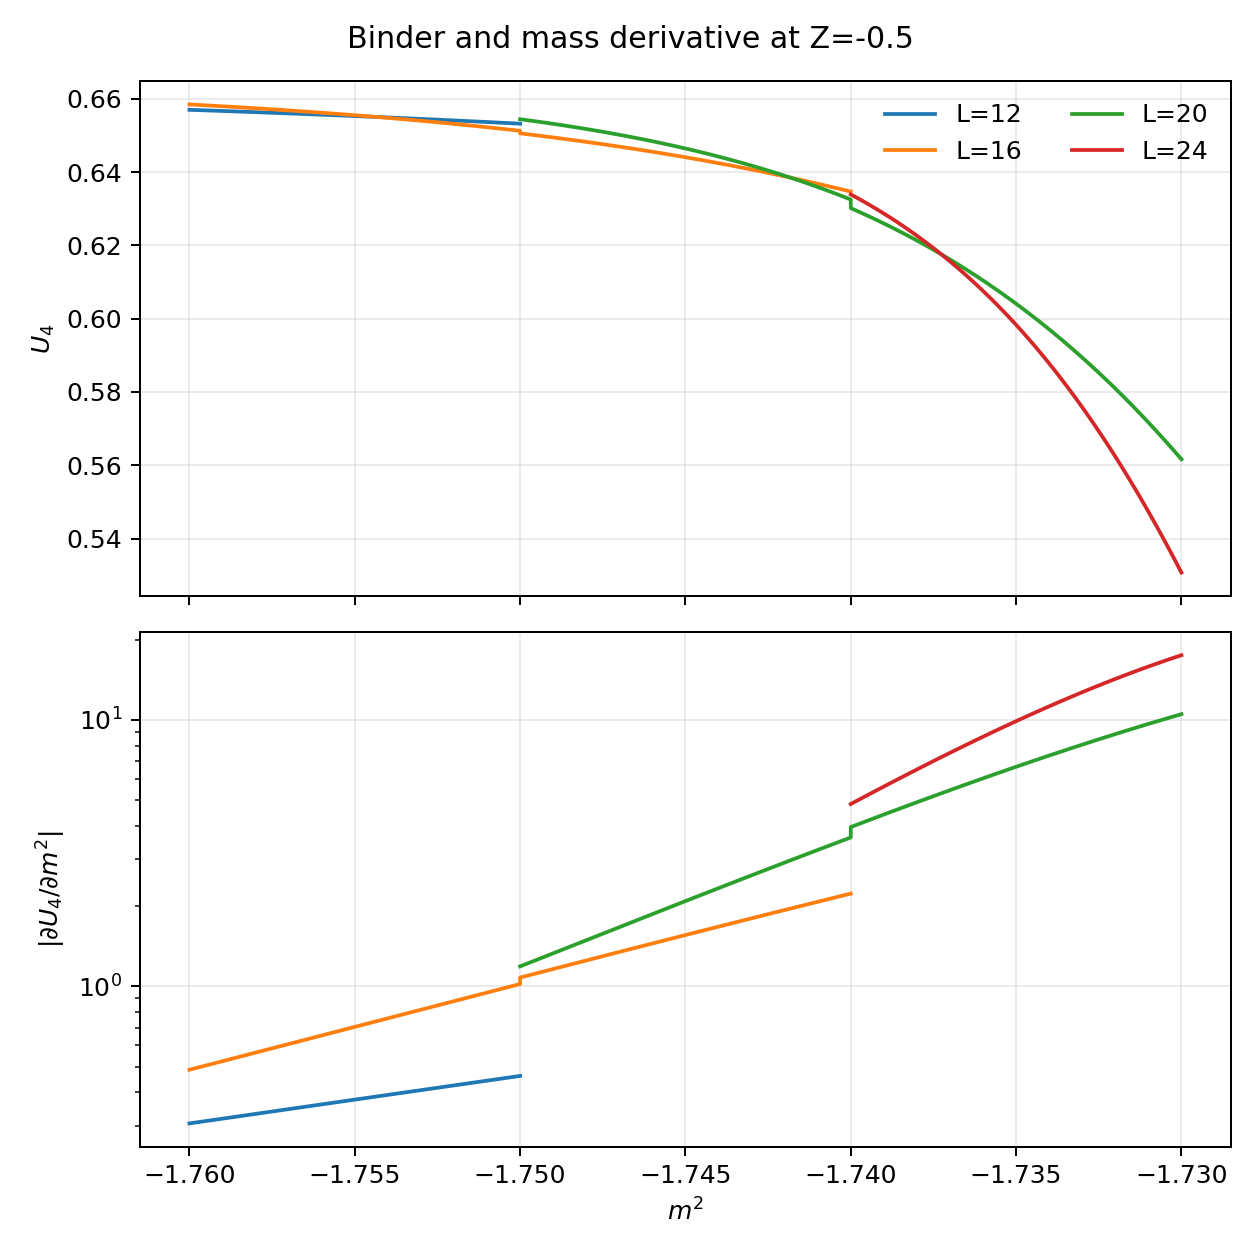
\includegraphics[width=0.77\linewidth]
  {../binder_slope_fss/preliminary/slope_curves_Zm0p5.png}
  \caption{Reconstructed Binder curves and analytic mass derivatives at
  $Z=-0.5$.  Each size-pair neighborhood is reconstructed from both endpoint
  masses and both phase starts.  Repeated size traces arise because a size can
  enter two adjacent-pair neighborhoods.}
  \label{fig:slope-zm05}
\end{figure}

The central-value validation pass gives the following $Z=-0.5$ sequence:
\begin{center}
\begin{tabular}{@{}cccc@{}}
\toprule
pair & refined $m_c^2$ & $y_{\mathrm{eff}}$ & diagnostic \\
\midrule
$12\times16$ & $-1.754317$ & $2.263$ & pass \\
$16\times20$ & $-1.741827$ & $1.866$ & pass \\
$20\times24$ & $-1.737262$ & $1.713$ & pass \\
\bottomrule
\end{tabular}
\end{center}
The downward drift is important: the smallest pair alone could look much more
singular than the largest pair.  The $20\times24$ central result lies near the
ordinary three-dimensional Ising thermal exponent
$y_t=1/\nu\simeq1.588$~\cite{Hasenbusch1999}, but this is not yet an exponent fit and the present
sizes do not justify a universality claim.  Across the other completed $Z$
campaigns, several phase-start discrepancies exceed the deliberately strict
$0.01$ Binder-spread threshold, and some legacy crossings do not remain
bracketed under local reweighting.  Those cases are flagged or excluded rather
than converted into effective exponents.

\begin{figure}[t]
  \centering
  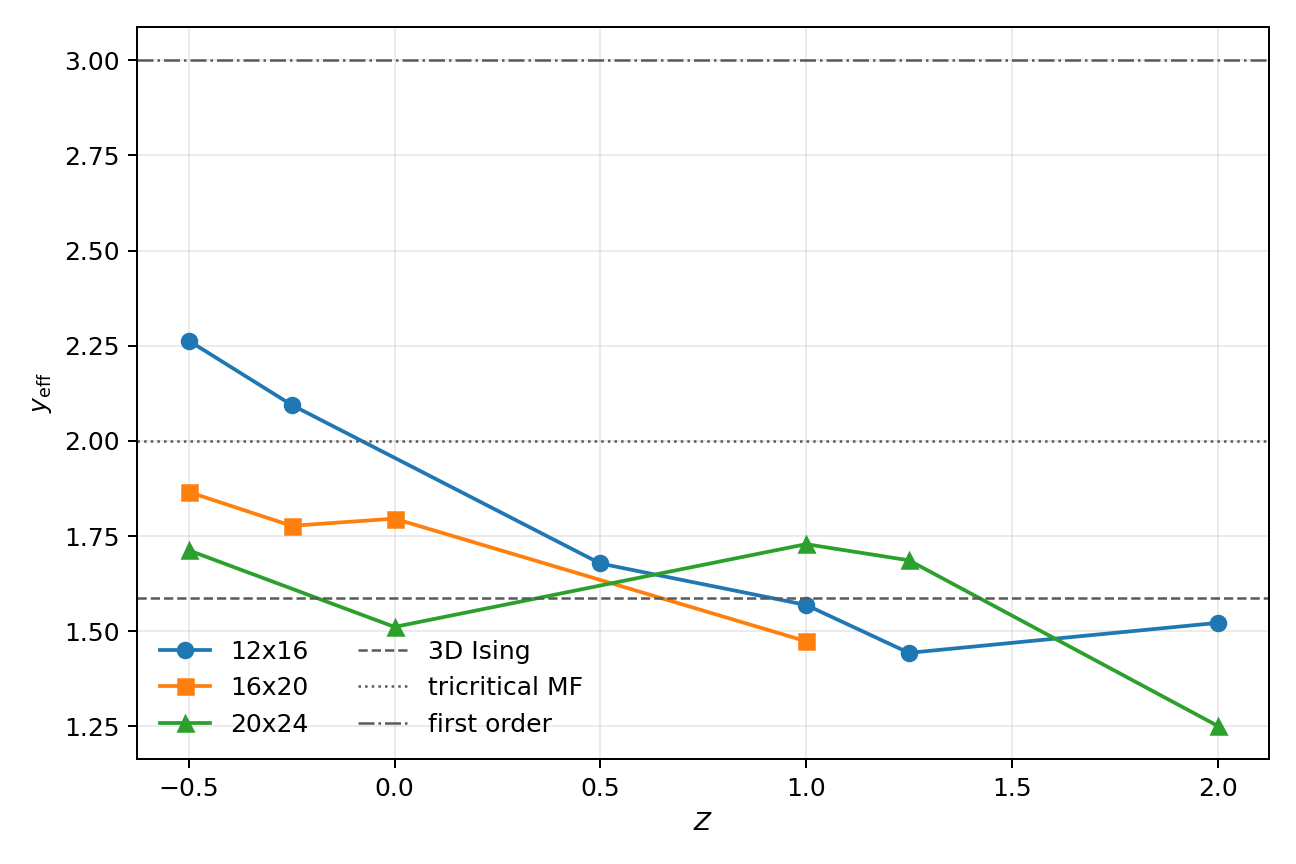
\includegraphics[width=0.75\linewidth]
  {../binder_slope_fss/preliminary/effective_exponents_vs_Z.png}
  \caption{Central finite-size effective exponents from refined crossings.
  Horizontal lines show conventional reference values only: 3D Ising
  $1/\nu$, mean-field tricritical $2$, and first-order volume scaling $3$.
  Missing pair--$Z$ points failed the local crossing-bracket test.  The
  one-draw validation intervals are intentionally omitted; production
  bootstrap intervals require the documented 200- and 500-draw runs.}
  \label{fig:yeff-z}
\end{figure}

These reference lines are benchmarks, not automatic labels.  Three-dimensional
tricritical scaling can carry logarithmic corrections because $d=3$ is its
upper critical dimension~\cite{Stephen1975}; near a modulated or Lifshitz
regime even the uniform magnetization and the conventional scaling fields may
be inappropriate.  A first-order conclusion would additionally require
coexistence or barrier evidence and a stable trend toward volume scaling.
The completed $Z=-0.75$ and $-1$ size sets will enter this analysis
automatically only after every manifest item for all four sizes is complete.

\section{Principal numerical and conceptual challenges}

\begin{enumerate}
  \item \textbf{Mismatch between umbrella coordinate and possible order.}
  Umbrella sampling in $M^2=|\phi(0)|^2$ is well aligned with uniform
  coexistence.  It may not accelerate tunneling among modulated states whose
  decisive coordinate is $|\phi(k\simeq\kstar)|^2$ or the orientation of
  $\kstar$.

  \item \textbf{Slow replica transport.}
  The number of windows and the round-trip time grow rapidly with $L$ and with
  the widened $M^2$ interval.  The unresolved endpoint tasks at $Z=-0.75$ and
  early $Z=-1$ stops are direct evidence that the chosen transport criterion
  is a binding constraint.

  \item \textbf{Commensurability.}
  On a periodic lattice, only $k_\mu=2\pi n_\mu/L$ is available.  A preferred
  $\qstar=-Z/2$ generally lies between momentum shells.  Shell changes as $L$
  varies can mimic irregular finite-size behavior and must be tracked
  explicitly.

  \item \textbf{Crossing ambiguity.}
  Nonmonotone or noisy curves can cross more than once.  Selecting the
  highest-$\Ufour$ crossing is reproducible, but its systematic uncertainty is
  not represented by the pair spread in Table~\ref{tab:crossings}.

  \item \textbf{Uncertainty model.}
  The present combined tables use one bootstrap pass; their quoted
  uncertainty reduces to the ordered/disordered source half-range.  Reliable
  confidence intervals require blocked resampling with enough independent
  effective samples, alongside autocorrelation and source-consistency checks.

  \item \textbf{First-order versus crossover signatures.}
  A Binder anomaly alone is not a first-order diagnostic.  Coexistence peaks,
  tunneling, free-energy barriers, latent-heat-like energy separation, and
  their volume or area scaling are required.
\end{enumerate}

\section{Recommended next analysis}

The immediate plan should preserve the present simple analysis while adding
the minimum observables needed to test its interpretation.

\begin{enumerate}
  \item Finish or explicitly classify every $Z=-0.75$ and $-1$ replica, then
  repeat the identical uniform-$M$ Binder analysis without tuning the crossing
  rule after seeing the result.

  \item Measure the structure factor
  \begin{equation}
    S(k)=\frac{1}{L^3}\left\langle |\phi(k)|^2\right\rangle
  \end{equation}
  and shell-average it in $q(k)$.  Test whether the dominant peak moves from
  $q=0$ toward $q\simeq -Z/2$ and whether its height scales with volume.

  \item Define a finite-wavevector order parameter from the dominant momentum
  shell, with its own susceptibility and Binder ratio.  Because the cubic
  lattice provides several symmetry-related wavevectors, the definition must
  account for shell degeneracy and orientational switching.

  \item Around the observed onset, perform a finer scan in $Z$ and $m^2$ and
  add distribution-based first-order tests: equal-weight peak matching,
  free-energy barrier growth (expected to scale as an interface area at a
  conventional first-order transition), and susceptibility maxima versus
  $L^3$.

  \item Only after these tests, fit competing finite-size scenarios.  Depending
  on the topology of the full phase diagram, the meeting point could be a
  critical endpoint, a tricritical point, or a Lifshitz-related multicritical
  structure; the present data do not select among them.
\end{enumerate}

\subsection{Implemented CPU structure-factor workflow}

The recommended structure-factor analysis is now implemented as a staged,
restartable CPU workflow.  It leaves the GPU production files read-only.  Its
first stage evaluates the full lattice Fourier spectrum of every available
equilibrated checkpoint at $Z=-1,-0.75,-0.5,0,$ and $0.5$.  Momenta are grouped
by the exact lattice invariant
\begin{equation}
  q(k)=4\sum_{i=1}^{3}\sin^2(k_i/2),
\end{equation}
and the measured dominant shell is frozen separately for each $(Z,L)$ before
examining the fine mass scan.  Consequently, $q\simeq -Z/2$ remains a plotted
mean-field reference rather than an imposed choice.

For the selected shell $\mathcal S_*$, production stores
\begin{equation}
  P_* = \sum_{k\in\mathcal S_*}\frac{|\phi(k)|^2}{V^2},
  \qquad
  S_* = \frac{V\langle P_*\rangle}{|\mathcal S_*|},
\end{equation}
together with the largest orientation fraction and an orientational
participation ratio.  The finite-wavevector Binder convention is
\begin{equation}
  U_* = 1-\frac{g}{g+2}
  \frac{\langle P_*^2\rangle}{\langle P_*\rangle^2},
  \qquad g=|\mathcal S_*|,
\end{equation}
which has a Gaussian-shell limit of zero.  The corresponding susceptibility,
energy density, $Q=\sum_x\phi_x^2$, and gradient invariant $G$ are retained in
the same joint sample.  This permits local reweighting in both $m^2$ and $Z$;
an effective-sample-size failure generates a request for a new simulation point
rather than an extrapolated claim.

Uncertainties use moving blocks of complete trajectories, keeping all umbrella
slots together and reconstructing the canonical umbrella weights in every
bootstrap draw.  Collection proceeds in 200-sample stages up to 1000 samples,
extending only tasks that fail the structure-factor, susceptibility, Binder,
overlap, or independent-source checks.  Distribution diagnostics test both
$\sqrt{P_*}$ and energy density for bin-stable coexistence peaks, equal-weight
matching, and barrier growth.  The implementation and generated provenance are
in \path{scripts/structure_factor_campaign.py},
\path{scripts/structure_factor_analysis.py}, and
\path{reports/structure_factor_cpu/}.

\subsection{Completed structure-factor campaign}

The staged campaign has now reached its preset cap.  It analyzed 114 independent
source runs: 99 required 200 retained trajectories, while the adaptive checks
extended selected source pairs through 400, 600, 800, and finally 1000
trajectories.  At the cap, 107 sources pass every overlap, within-source
precision, and ordered/disordered agreement gate.  The seven nonpassing sources
are confined to $Z=-1$: both sources at $(L,m^2)=(16,-2.52)$ and the selected
sources at $L=20$, $m^2=-2.56,-2.55,-2.54$.  Their only failed diagnostic is
persistent ordered/disordered source disagreement.  No further automatic
extension is allowed beyond 1000 trajectories.

Figure~\ref{fig:selected-shell} shows the shell choice made before production.
The controls and the $Z=-0.75$ and $-0.5$ scans select $q_*=0$ for every available
size.  At $Z=-1$, the selected shell changes from $q_*=0$ at $L=12$ to the
smallest nonzero lattice shell,
\begin{equation}
  q_*(16)=0.152240934977,
  \qquad q_*(20)=0.097886967410.
\end{equation}
Both are far below the bare mean-field guide $-Z/2=0.5$.  This displacement is
therefore a measured long-wavelength effect, not an imposed mean-field feature.
There is no completed $Z=-1$, $L=24$ source in the present campaign.

\begin{figure}[htbp]
  \centering
  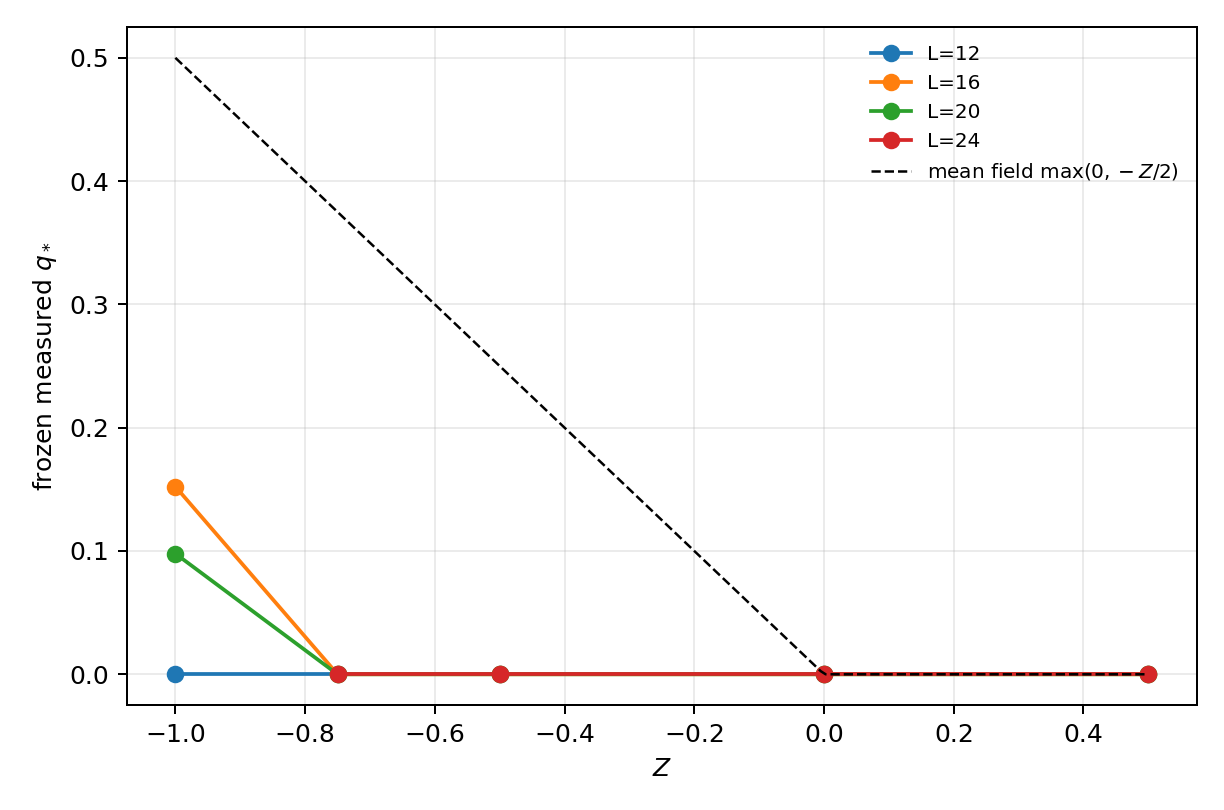
\includegraphics[width=0.72\textwidth]{../structure_factor_cpu/preparation/figures/selected_shell_vs_Z.png}
  \caption{Measured shell frozen for each $(Z,L)$.  The dashed line is the bare
  mean-field guide and is not used in shell selection.}
  \label{fig:selected-shell}
\end{figure}

At $Z=-1$, the nonzero-shell observables are qualitatively distinct from the
uniform controls.  Across the three selected masses, $S(q_*)$ per mode is
$69.7$--$73.1$ for $L=16$ and $123.2$--$142.0$ for $L=20$.  The shell Binder
ratio is strongly negative, approximately $-0.36$ to $-0.30$, and the
orientational participation ratio is close to two.  The ordered/disordered
$S(q_*)$ separation remains much larger than the blocked-bootstrap error at the
1000-trajectory cap: the separation-to-combined-error ratios are approximately
$25.8$ at $(16,-2.52)$ and $2.9$, $5.7$, and $16.0$ at the three $L=20$ masses.
Figure~\ref{fig:finite-q-zm1} summarizes these finite-wavevector observables.

\begin{figure}[htbp]
  \centering
  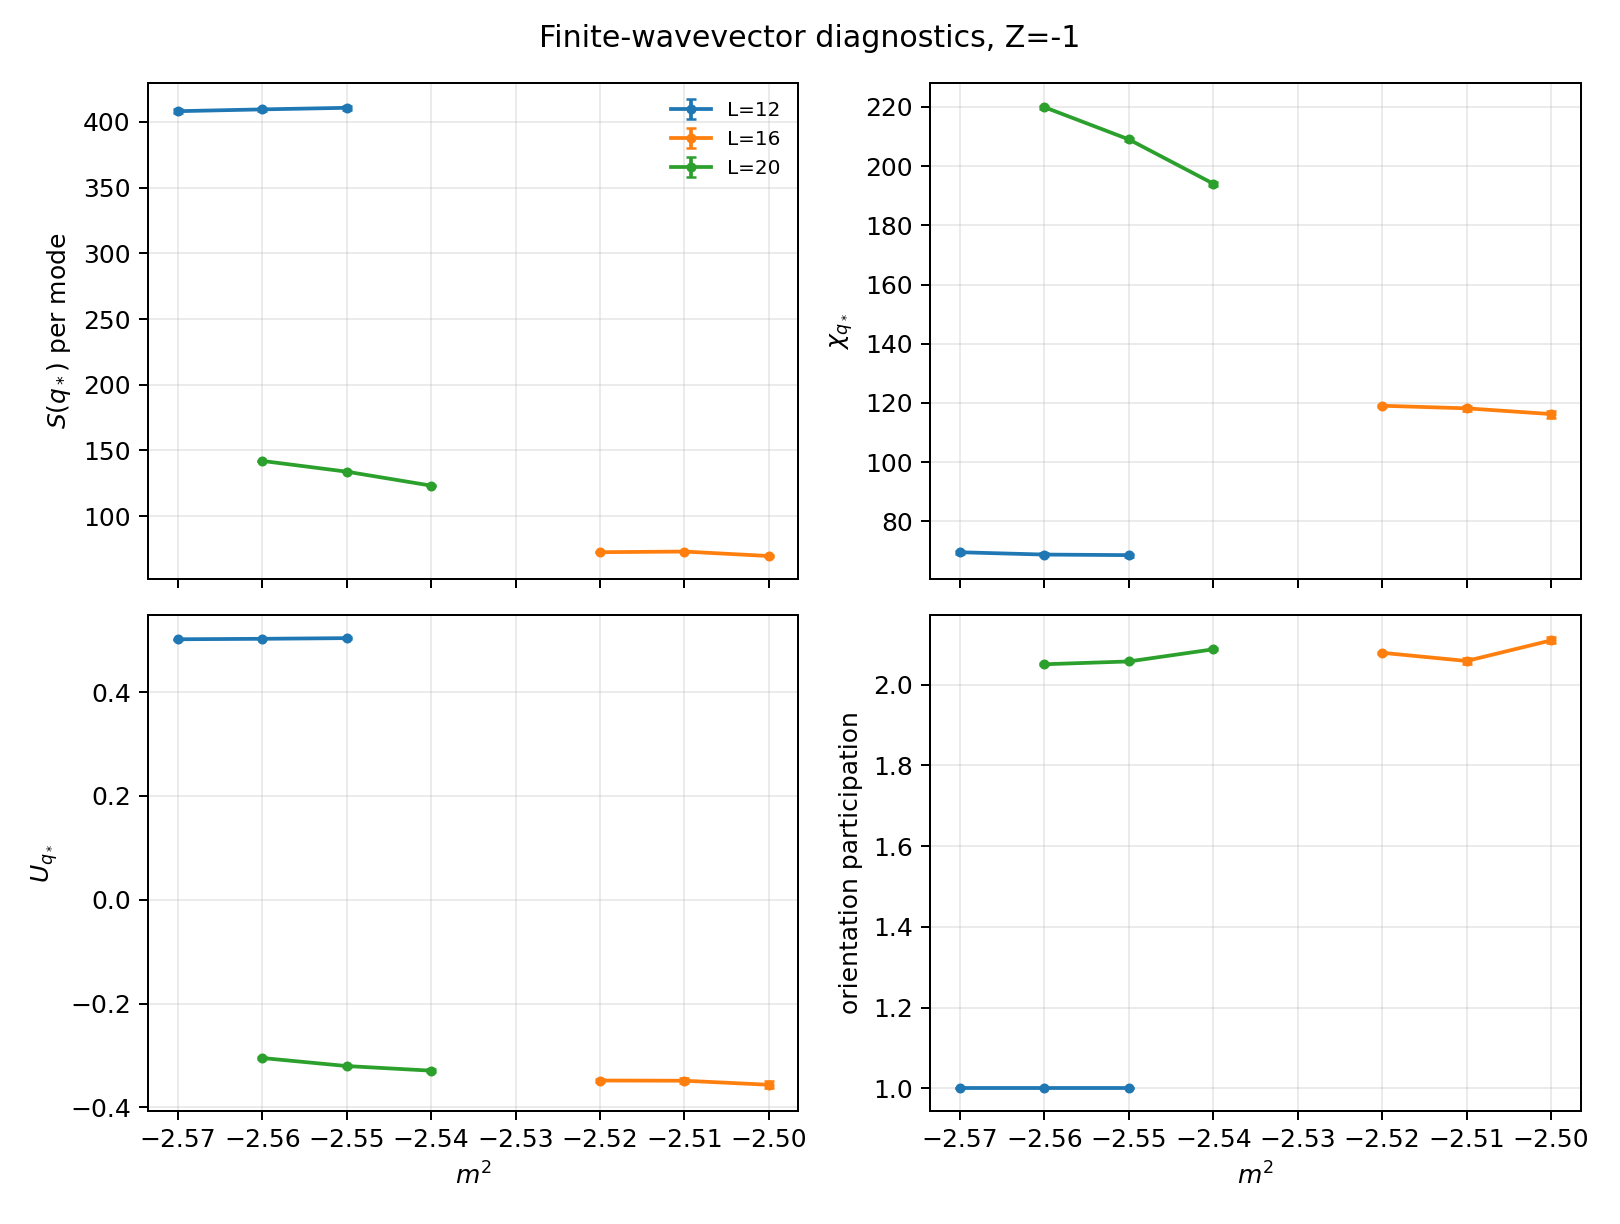
\includegraphics[width=0.86\textwidth]{../structure_factor_cpu/analysis/figures/finite_q_Zm1p0.png}
  \caption{Finite-wavevector observables at $Z=-1$.  Error bars are blocked
  bootstrap uncertainties; independent source separation is retained as a
  separate diagnostic and is the limiting systematic at $L=16,20$.}
  \label{fig:finite-q-zm1}
\end{figure}

The distribution tests do not yet establish a conventional first-order
transition.  Several individual $Z=-1$ sources have bin-stable two-peak
structure in the shell amplitude, with central-point barriers up to about
$2.4$, but the peak weights are generally unequal and no central $Z=-1$ source
has bin-stable energy bimodality.  Small energy double-peak fits found in some
$Z=0$ controls have barriers below $0.72$, illustrating why histogram shape
alone is insufficient.  Moreover, the selected mass windows differ between
$L=16$ and $20$, so the present points do not support a controlled volume- or
interface-scaling fit.

The conservative interpretation is therefore: the campaign gives direct
evidence that the uniform order parameter becomes inadequate at $Z=-1$ and
locates a long-wavelength, history-dependent regime consistent with an
inhomogeneous or strongly metastable phase.  It does not yet distinguish a
first-order boundary from slow phase mixing or another finite-size mechanism.
The decisive follow-up is a dedicated $Z=-1$, $L=24$ run and a finer common
$(Z,m^2)$ grid around this onset, followed by equal-weight and barrier scaling
using the same frozen-shell convention.

As a direct calibration of the estimator, a deliberately deep modulated point
was also tested at $(Z,m^2,L)=(-4,-1,16)$.  Here the bare minimum $q=-Z/2=2$
is exactly an axial lattice shell with wavelength four sites.  Averaging exact
stripe configurations over all three axes and several phases leaves a unique
shell-power peak at $q=2$, because the estimator sums $|\phi(k)|^2$ over the
shell before ensemble averaging.  An HMC run initialized in one stripe,
comprising 1000 warmup trajectories and 200 retained configurations, likewise
peaks at $q=2$ with 93.8\% measurement acceptance.  Its peak is approximately
$5.7\times10^3$ times the next-largest shell, and the mean largest-orientation
fraction is $0.99989$.  Figure~\ref{fig:deep-modulated-validation} therefore
rules out cancellation by orientational or phase averaging as the explanation
for the subtler $Z=-1$ result.

\begin{figure}[htbp]
  \centering
  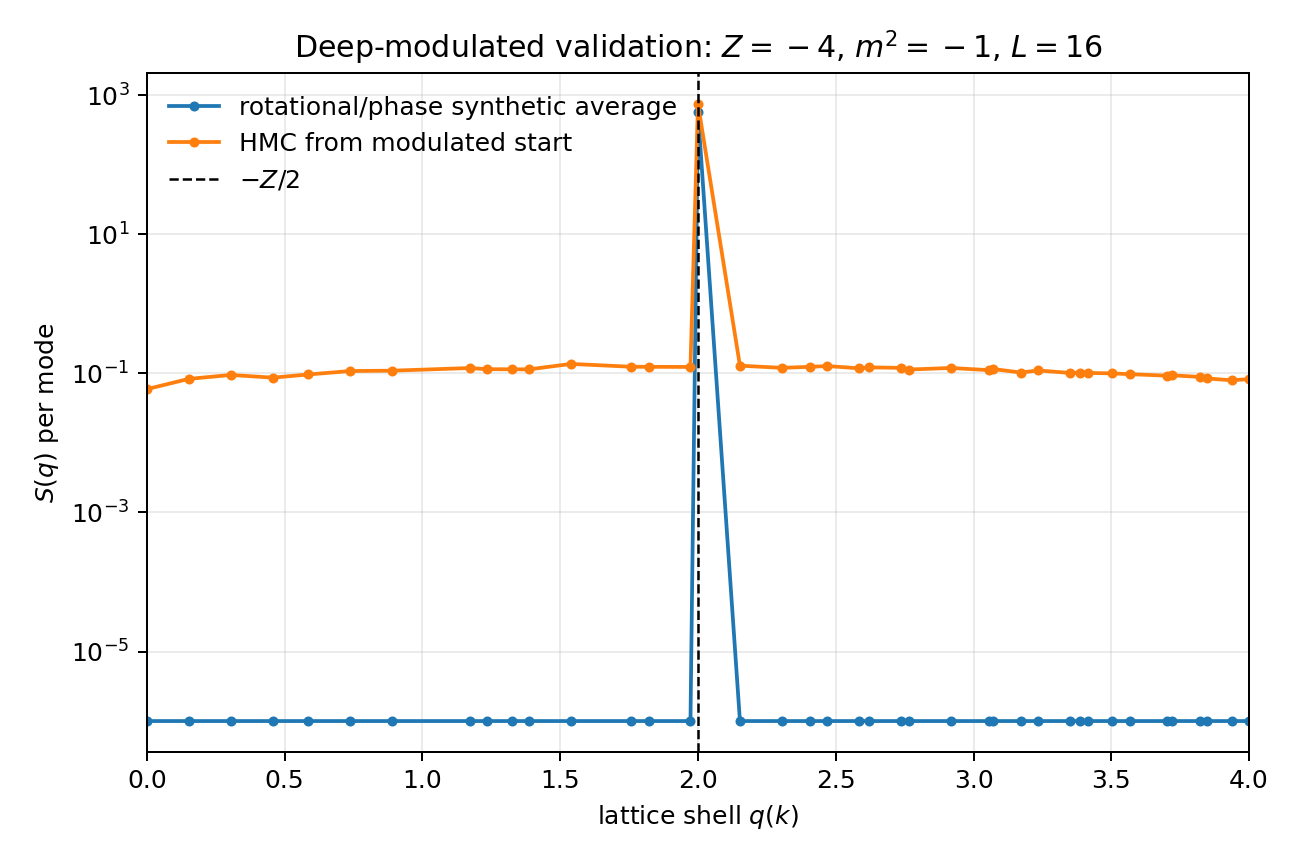
\includegraphics[width=0.78\textwidth]{../structure_factor_cpu/deep_modulated_validation/spectrum_validation.png}
  \caption{Deep-modulated calibration.  Both the synthetic rotational/phase
  average and the equilibrated HMC sample recover the imposed $q=2$ shell.}
  \label{fig:deep-modulated-validation}
\end{figure}

\subsection{Wide $L=16$ continuation map in $(Z,m^2)$}

The deep-modulated calibration establishes that the estimator can detect a
strong finite-wavevector state, but it does not locate where such a state first
becomes competitive.  We therefore performed an exploratory $L=16$ CPU scan
over a substantially wider parameter patch.  The coarse grid covers
$Z=-0.5,-0.625,\ldots,-3$; the suspected onset interval
$-2.50\leq Z\leq-2.25$ is resolved more finely with $\Delta Z=0.025$.
At every $Z$, the $m^2$ grid has spacing $0.25$ and contains the exact mass
obtained by quadratically extrapolating the available Binder-crossing line.
The high-mass endpoint satisfies
$m^2_{\rm high}\geq Z^2/4+1$ so that it lies above the bare finite-$q$
instability.  For $Z\leq-2.3$, the low endpoint is four mass units below that
extrapolated line.

Three continuations are followed on each mass grid: a uniform ordered start,
a single-mode start on the lattice shell nearest the bare guide $-Z/2$, and a
high-mass disordered start continued downward.  The last continuation is only
disordered near its starting endpoint; at lower mass it may settle into a
different ordered momentum shell.  For any two such restricted branches
$a,b$, the free-energy-density difference obeys
\begin{equation}
  \frac{\partial(f_a-f_b)}{\partial m^2}
  =\frac{1}{2}\left(\frac{\langle Q\rangle_a}{V}
  -\frac{\langle Q\rangle_b}{V}\right),
  \qquad Q=\sum_x\phi_x^2.
  \label{eq:branch-ti}
\end{equation}
The branches are assigned equal free energy at the high-mass endpoint and
Eq.~\eqref{eq:branch-ti} is integrated downward by the trapezoid rule.  At each
mass, the finite-$q$ envelope is the lower of the two coherent nonzero-shell
continuations; an operational requirement $S_{\rm peak}\geq10$ prevents
noise-level shell labels from defining a boundary.

The final manifest contains 29 $Z$ slices, 1142 mass points, and 3426 branch
measurements.  The minimum HMC acceptance is $0.90$ and the mean is $0.974$.
Figure~\ref{fig:wide-phase-map} shows the resulting two-dimensional map.  From
$Z=-0.5$ through $-2.275$, the uniform continuation remains lower on the
extrapolated Binder line.  At $Z=-2.300$, the coherent finite-$q$ envelope is
already lower.  The finite-volume onset is consequently bracketed by
\begin{equation}
  -2.300 \leq Z_{\rm onset}(L=16) < -2.275.
  \label{eq:onset-bracket}
\end{equation}
The central differences $\Delta f=f_{q>0}-f_{q=0}$ on this line change from
$+0.0135$ at $Z=-2.275$ to $-0.0694$ at $Z=-2.300$.

\begin{table}[htbp]
  \centering
  \caption{Restricted finite-$q$ envelope evaluated on the extrapolated
  Binder line near the $L=16$ onset.  Negative $\Delta f$ favors the indicated
  coherent finite-$q$ continuation.}
  \label{tab:wide-onset}
  \begin{tabular}{rrrr}
    \toprule
    $Z$ & $m^2_{\rm Binder,ext}$ & $\Delta f$ & selected $q$ \\
    \midrule
    $-2.250$ & $-5.775$ & $+0.0257$ & $1.1716$ \\
    $-2.275$ & $-5.857$ & $+0.0135$ & $1.1716$ \\
    $-2.300$ & $-5.941$ & $-0.0694$ & $1.2346$ \\
    $-2.325$ & $-6.025$ & $-0.0241$ & $1.1716$ \\
    $-2.350$ & $-6.110$ & $-0.0432$ & $1.1716$ \\
    $-2.375$ & $-6.195$ & $-0.0462$ & $1.1716$ \\
    $-2.400$ & $-6.282$ & $-0.0958$ & $1.2346$ \\
    \bottomrule
  \end{tabular}
\end{table}

\begin{figure}[htbp]
  \centering
  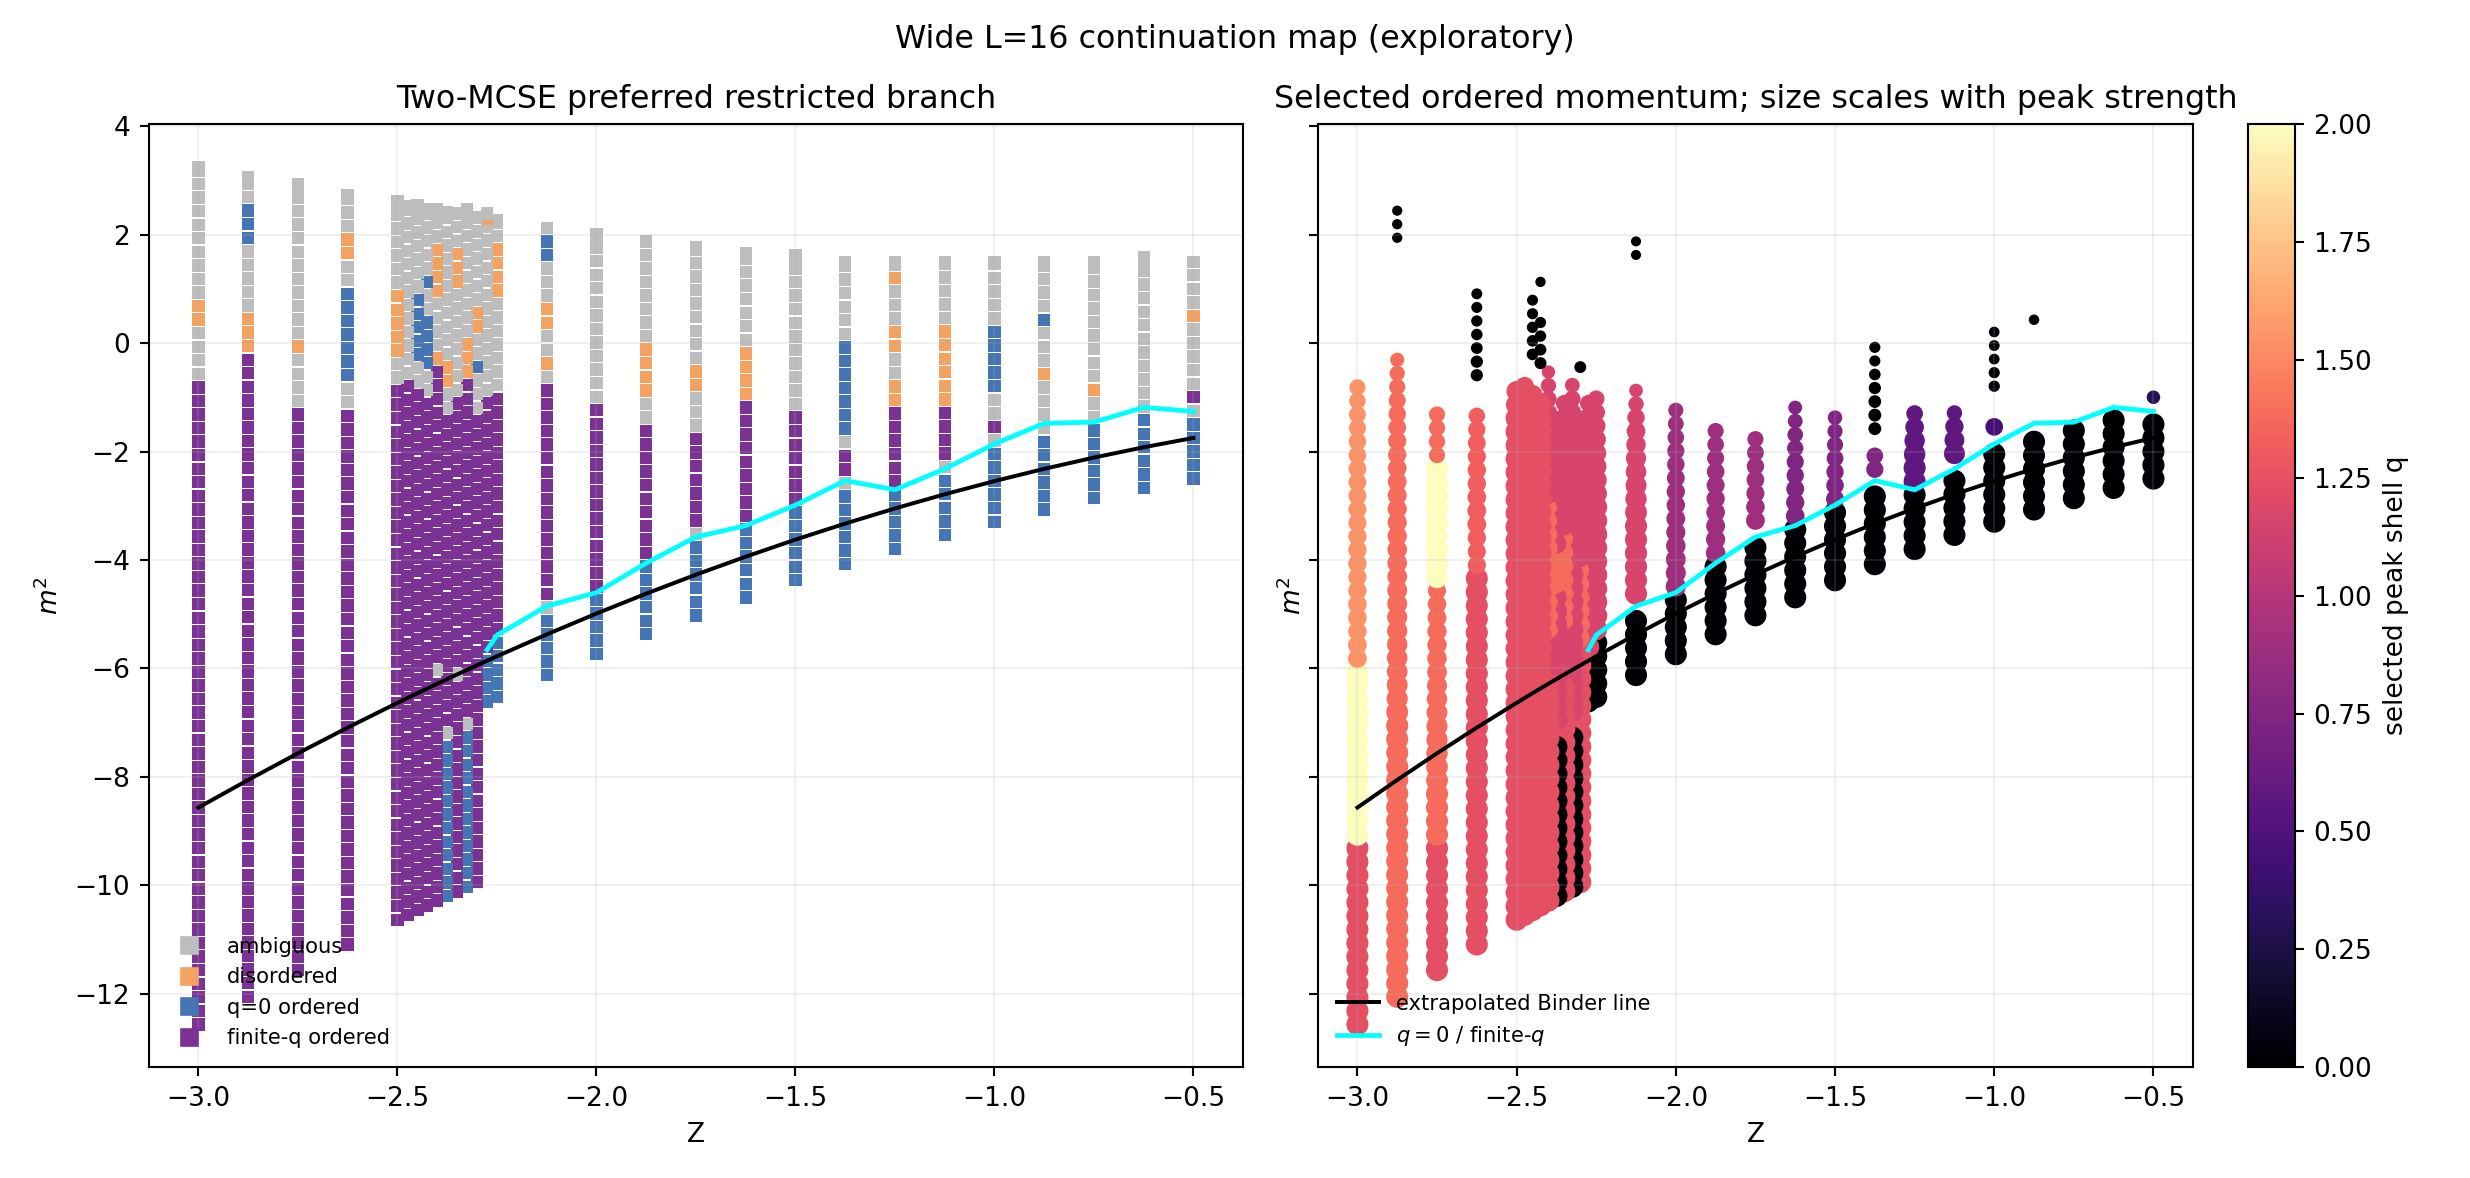
\includegraphics[width=0.98\textwidth]{../structure_factor_cpu/thermodynamic_integration_L16_wide/wide_phase_map.png}
  \caption{Wide $L=16$ continuation map.  Left: branch favored by more than
  two propagated MCSEs.  Right: momentum shell of the favored coherent
  ordered continuation; marker size grows with peak strength.  The black curve
  is the quadratic extrapolation of the existing Binder line and the cyan
  curve is the bracketed $q=0$/finite-$q$ restricted-branch crossing.}
  \label{fig:wide-phase-map}
\end{figure}

Figure~\ref{fig:wide-ti} exposes the principal finite-volume limitation.  The
selected shell jumps from $q=1.1716$ at $Z=-2.275$ to $q=1.2346$ at
$Z=-2.300$, precisely where Eq.~\eqref{eq:onset-bracket} changes sign.  At
larger $|Z|$, distinct coherent shells repeatedly exchange stability, and in
several slices a finite-$q$ continuation remains favored even at the extended
low-mass edge.  The jagged boundary is therefore valuable evidence for
finite-wavevector competition, but it cannot be interpreted as a smooth
thermodynamic phase boundary.  A linear interpolation would give
$Z\simeq-2.279$, but quoting it as a critical coupling would conceal the shell
locking that dominates this $L=16$ estimate.

\begin{figure}[htbp]
  \centering
  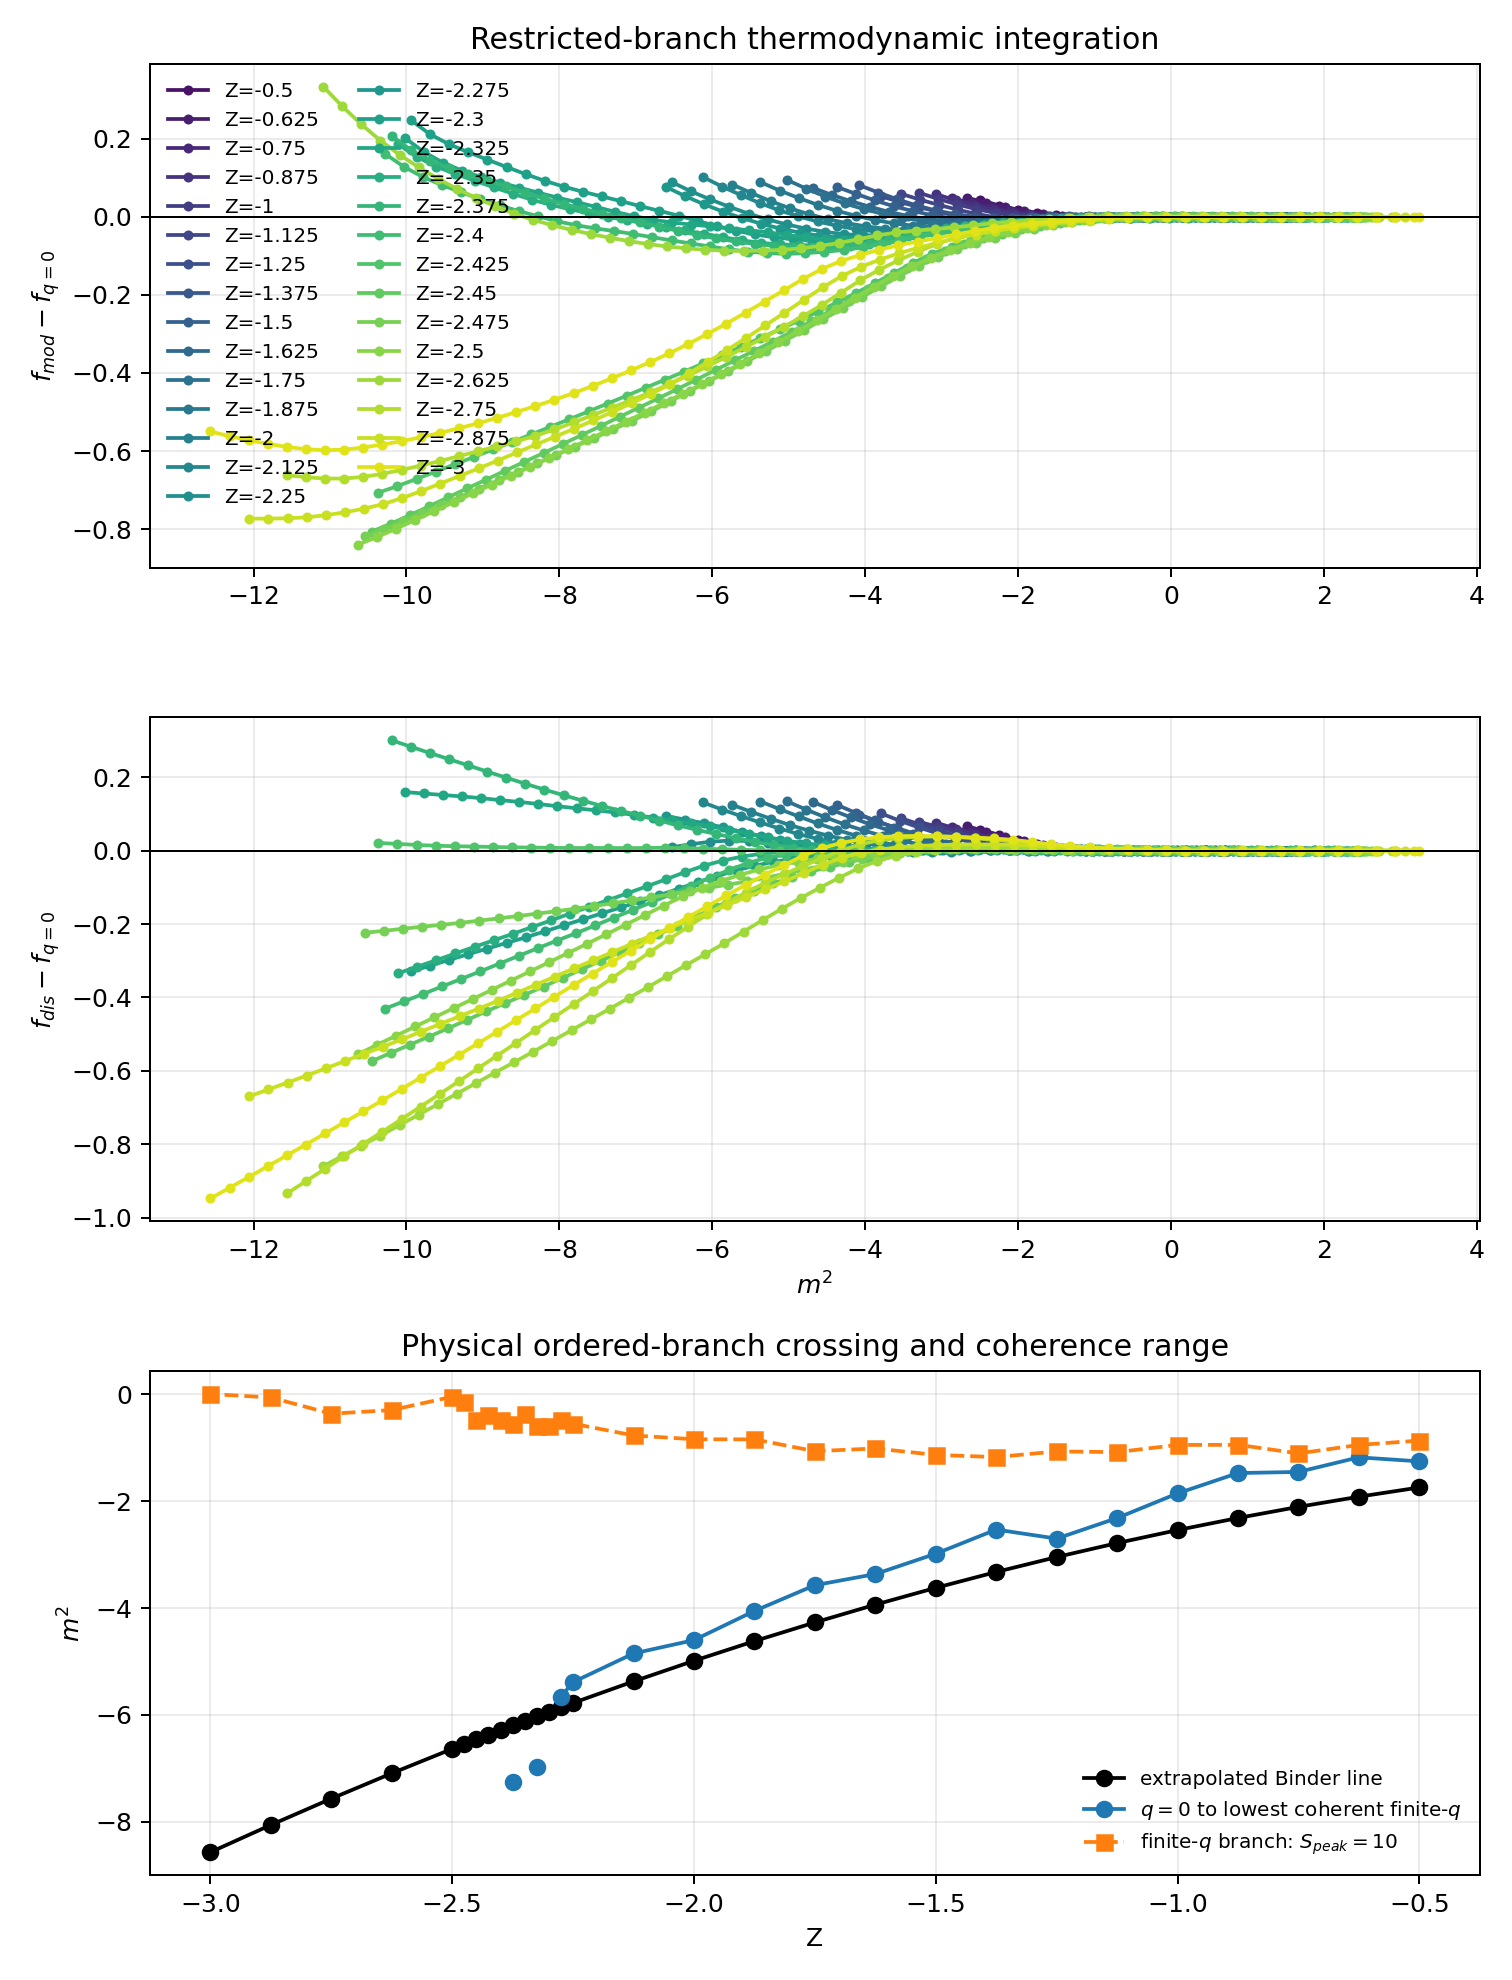
\includegraphics[width=0.82\textwidth]{../structure_factor_cpu/thermodynamic_integration_L16_wide/thermodynamic_integration.png}
  \caption{Restricted-branch thermodynamic integration.  The upper panels
  compare the initialized finite-$q$ and high-mass continuations with the
  uniform continuation.  The lower panel compares the filtered finite-$q$
  envelope with the extrapolated Binder line.  Roots in the high-mass merged
  regime are excluded from the filtered boundary.}
  \label{fig:wide-ti}
\end{figure}

The $L=16$ calculations are deliberately diagnostic.  They use one short
continuation per branch, and their batch-MCSE propagation does not include
initialization, continuation, or branch-selection systematics.

\subsection{$L=20$ finite-size and replica check}

To test whether Eq.~\eqref{eq:onset-bracket} survives a change of momentum
grid, the interval was repeated at $L=20$ for
$Z=-2.25,-2.2625,\ldots,-2.325$.  Two statistically independent continuation
replicas were run at every $Z$, each with the same three-branch construction
and a mass range extending four units below the extrapolated Binder line and
above $Z^2/4+1$.  The volume-scaled HMC choice
$\epsilon=0.0085$, $n_{\rm lf}=15$ gives a minimum acceptance of $0.897$ and a
mean of $0.975$.  The campaign contains 712 mass points and 2136 branch
measurements.

The result is qualitatively different from $L=16$.  In both $L=20$ replicas,
the finite-$q$ envelope remains above the uniform continuation at every
extrapolated Binder-line mass.  Replica~0 gives
$0.0282\leq\Delta f\leq0.0392$ and replica~1 gives
$0.0318\leq\Delta f\leq0.0363$, with no sign change.  Both independently
select the same coherent shell,
\begin{equation}
  q_*(L=20)=1.14589803375,
\end{equation}
throughout the interval.  Their $q=0$/finite-$q$ restricted-branch crossings
occur at less-negative masses, approximately $m^2=-5.27$ to $-5.62$, whereas
the extrapolated Binder line spans approximately $-5.77$ to $-6.03$.

Figure~\ref{fig:l16-l20-onset} makes the finite-size discrepancy explicit.
The sharp $L=16$ sign reversal is accompanied by jumps among its allowed
shells; neither feature appears in the two $L=20$ replicas.  Consequently, the
$L=16$ bracket in Eq.~\eqref{eq:onset-bracket} does not survive the first
finite-size check.  This does not exclude a finite-$q$ boundary at more
negative $Z$ for $L=20$, but it rules out treating $Z\simeq-2.29$ as a
volume-stable onset.

\begin{figure}[htbp]
  \centering
  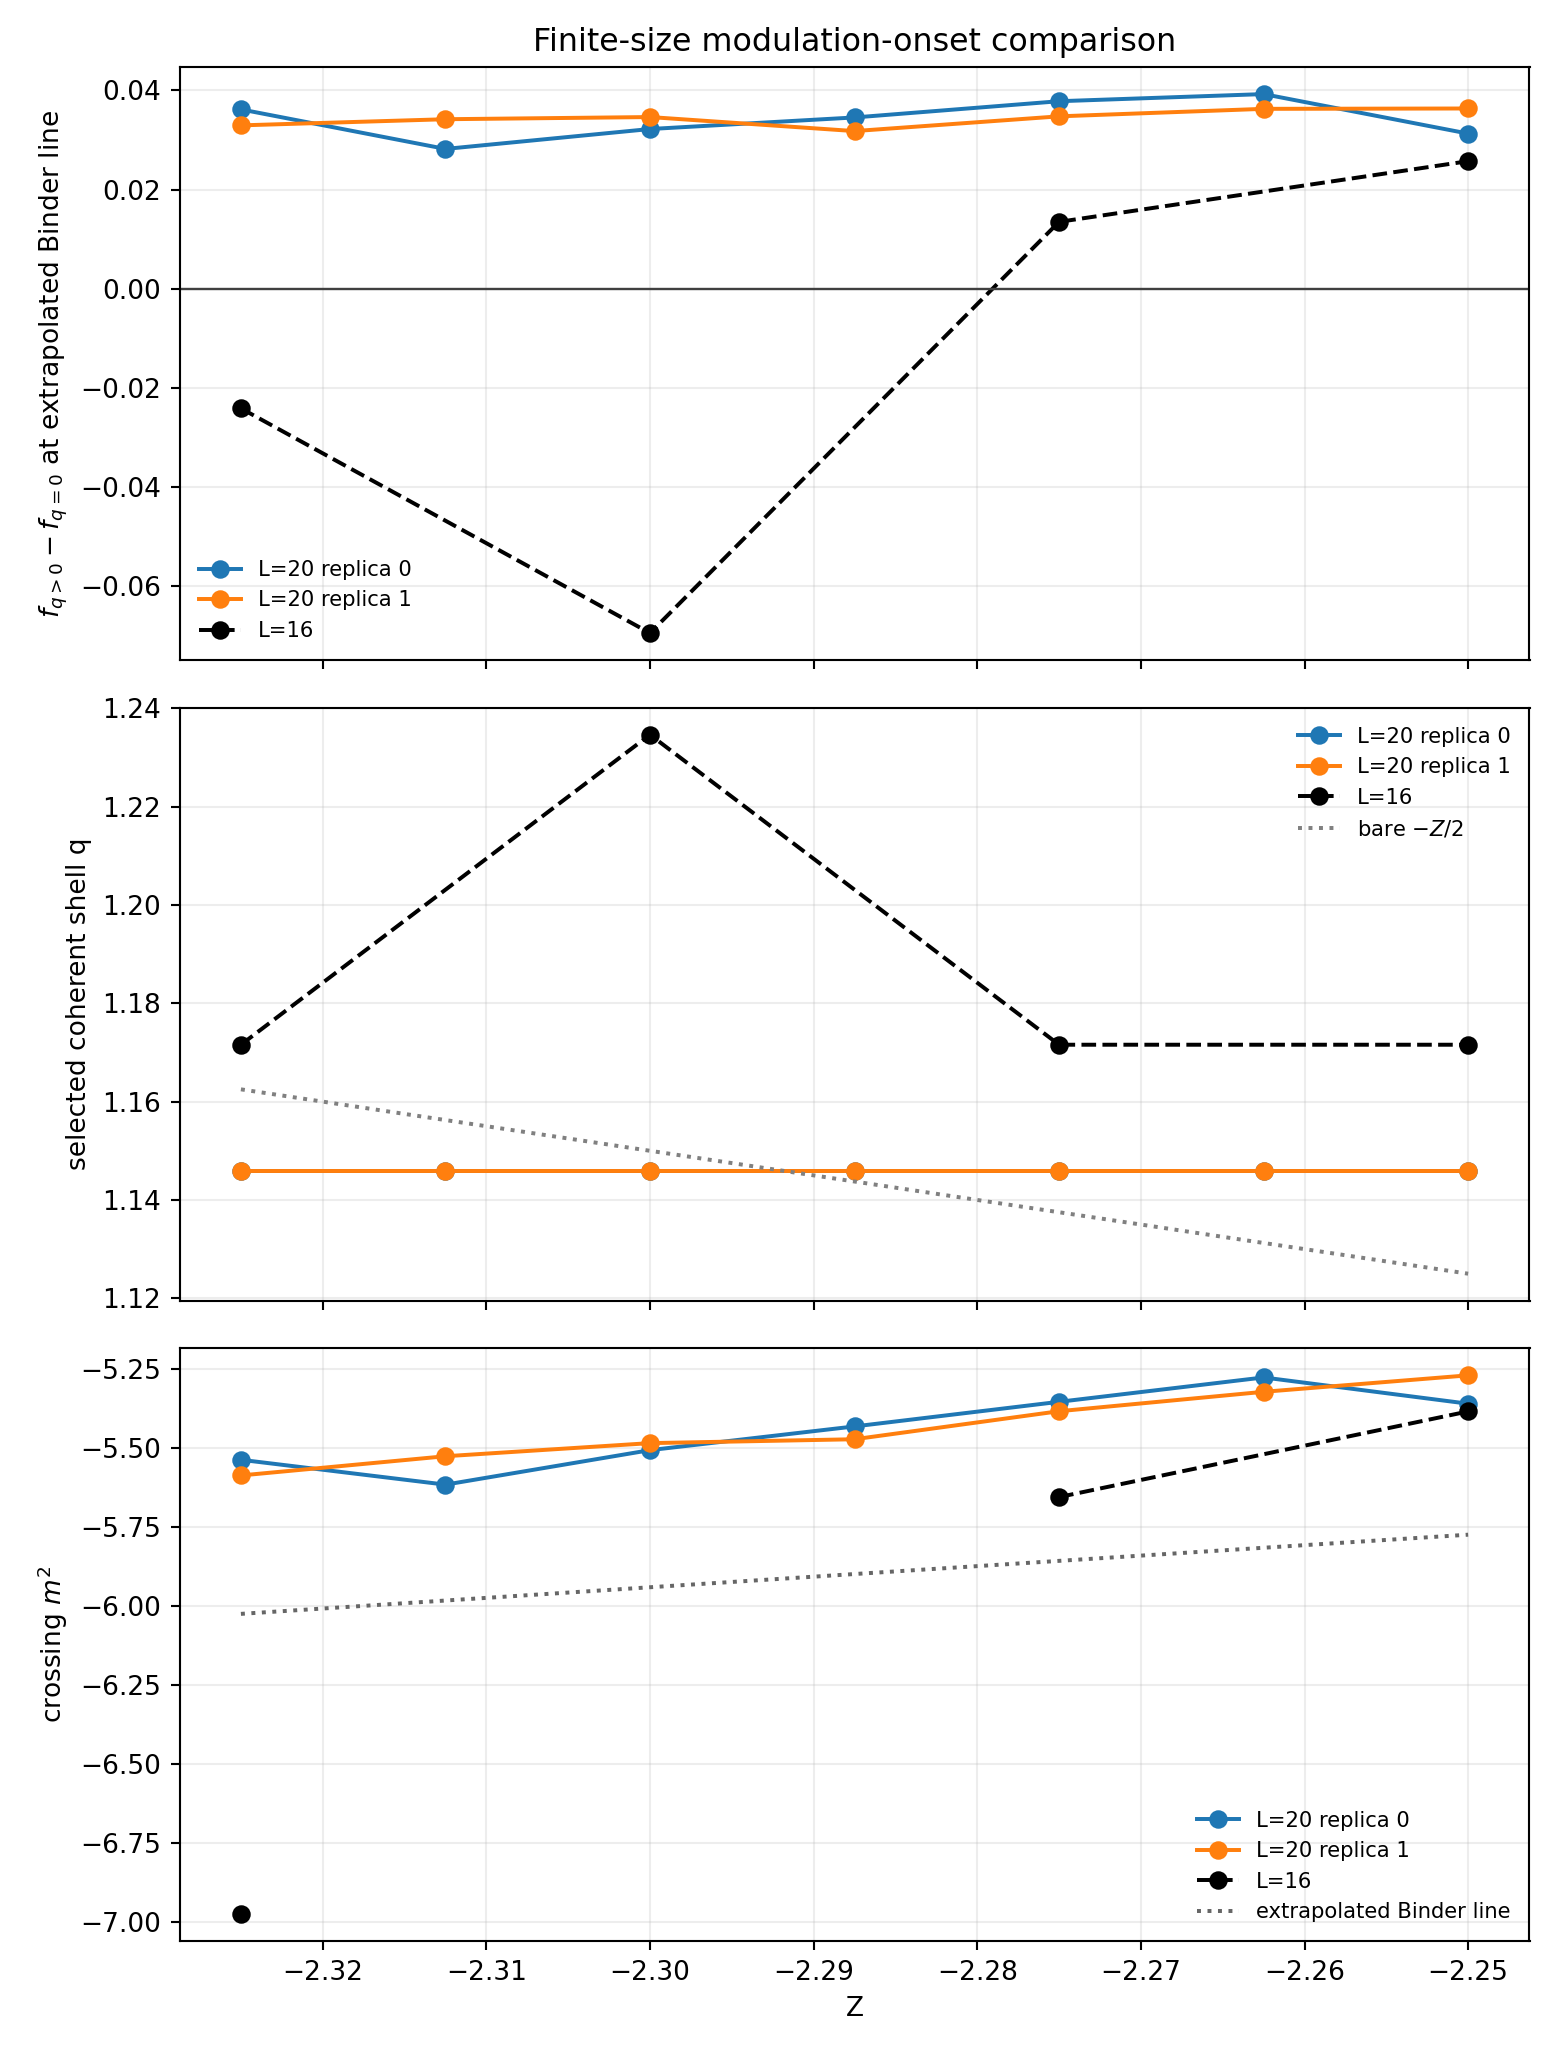
\includegraphics[width=0.84\textwidth]{../structure_factor_cpu/thermodynamic_integration_L20_onset/L16_L20_onset_comparison.png}
  \caption{Finite-size check of the apparent $L=16$ onset.  Top: restricted
  finite-$q$ minus uniform free energy on the extrapolated Binder line.
  Middle: selected coherent shell.  Bottom: restricted-branch crossing mass.
  The two independent $L=20$ replicas agree with each other and show no sign
  change over the interval in which $L=16$ changes sign.}
  \label{fig:l16-l20-onset}
\end{figure}

\subsection{Wide $L=20$ map and replicated shell threshold}

The $L=20$ scan was then extended across the full range $-3\leq Z\leq-0.5$.
It uses $\Delta Z=0.125$ from $-0.5$ to $-2.25$, $\Delta Z=0.025$ for
$-2.60\leq Z\leq-2.25$, and $\Delta Z=0.05$ from $-2.65$ to $-3$.
Its 37 slices contain 1640 mass points and 4920 branch measurements, with
minimum and mean acceptances $0.890$ and $0.976$.
Figure~\ref{fig:l20-wide}
shows that a finite-$q$ continuation is eventually favored on the extrapolated
Binder line, but the boundary is again jagged and correlated with changes of
the selected lattice shell.

On the larger-$Z$ side, the Binder-line point remains on the uniform side from
$Z=-0.5$ through $-1.5$.  Isolated negative differences occur at
$Z=-1.625,-1.875,$ and $-2.125$, but positive values return at the interleaved
points $Z=-1.75,-2,$ and $-2.25$.  These alternating signs follow changes of
the selected discrete shell and do not constitute a monotone onset line.

The first wide-scan sign change occurs between $Z=-2.350$ and $-2.375$:
\begin{equation}
  \Delta f(-2.350)=+0.0288,
  \qquad
  \Delta f(-2.375)=-0.0496.
\end{equation}
Simultaneously, the selected shell changes from
$q_1=1.14589803375$ to $q_2=1.20639550666$.  This interval was therefore rerun
with two fresh replicas at spacing $\Delta Z=0.005$.  Both switch sign between
$Z=-2.350$ and $-2.355$, giving interpolated roots
\begin{equation}
  Z_1=-2.3520763,
  \qquad
  Z_2=-2.3520854.
  \label{eq:l20-shell-roots}
\end{equation}
The nearest-shell midpoint predicts
\begin{equation}
  Z_{\rm shell}=-(q_1+q_2)=-2.3522935,
  \label{eq:l20-shell-midpoint}
\end{equation}
only about $2.1\times10^{-4}$ away.  Figure~\ref{fig:l20-refine} shows that the
free-energy sign and selected shell change on the same grid step in both
replicas.  The sharp crossing is consequently controlled by the discrete
$L=20$ momentum grid and the branch initialization/selection rule.  The wide
map still establishes a region in which finite-$q$ continuations are favored,
but it does not provide a smooth physical onset line.

\begin{figure}[htbp]
  \centering
  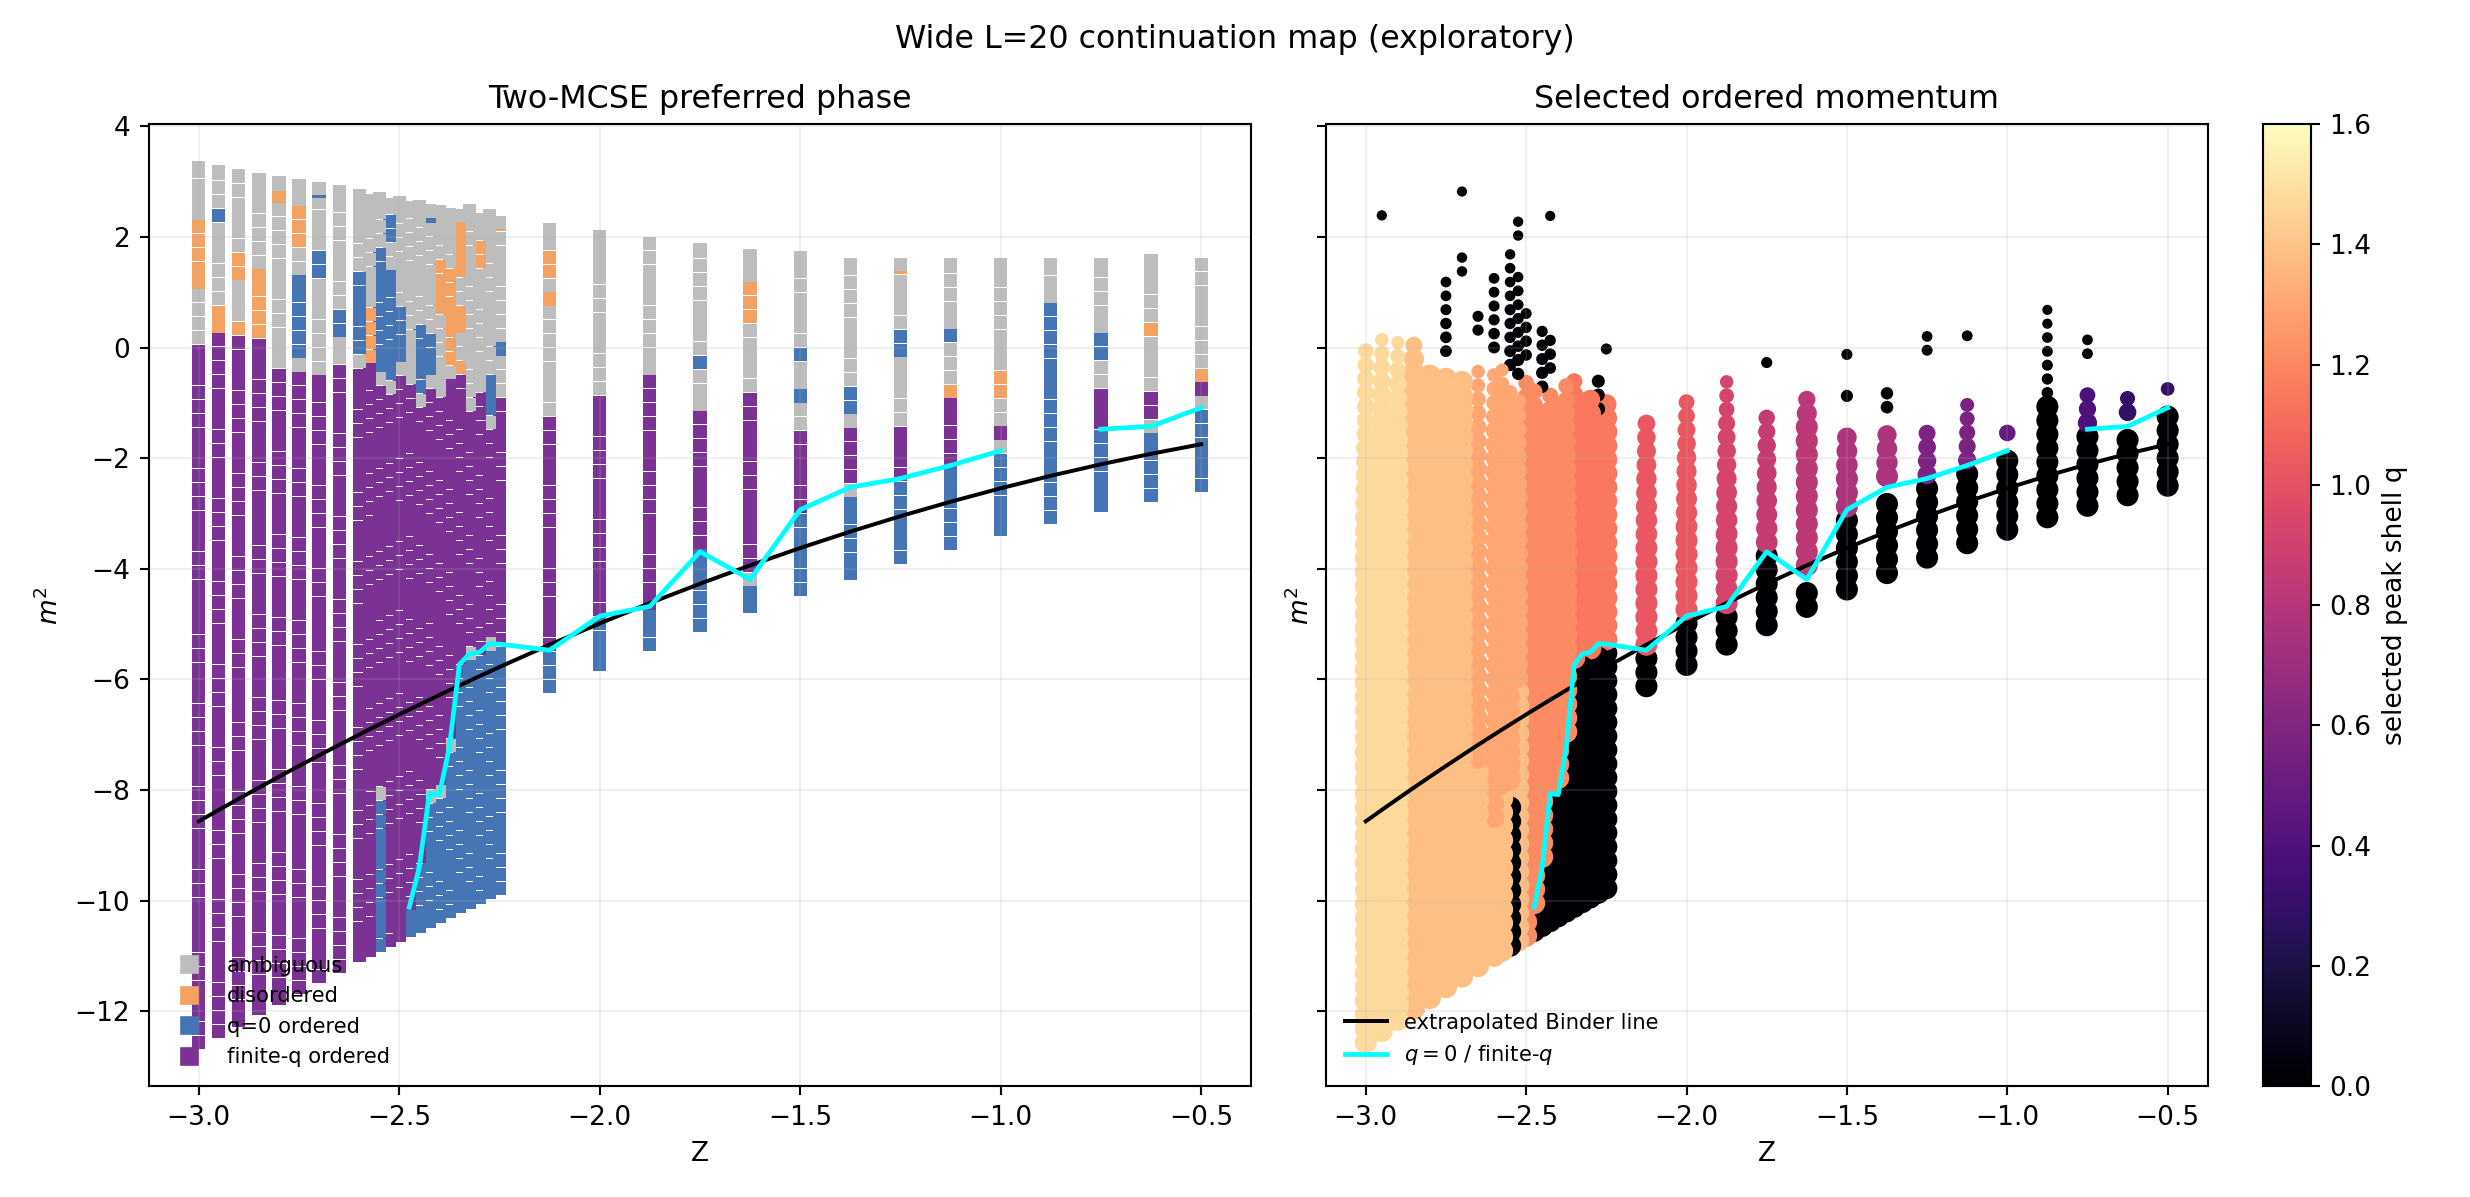
\includegraphics[width=0.98\textwidth]{../structure_factor_cpu/thermodynamic_integration_L20_wide/wide_phase_map.png}
  \caption{Wide $L=20$ continuation map.  The finite-$q$ region expands at
  negative $Z$, but its inferred boundary changes abruptly when the selected
  discrete momentum shell changes.}
  \label{fig:l20-wide}
\end{figure}

\begin{figure}[htbp]
  \centering
  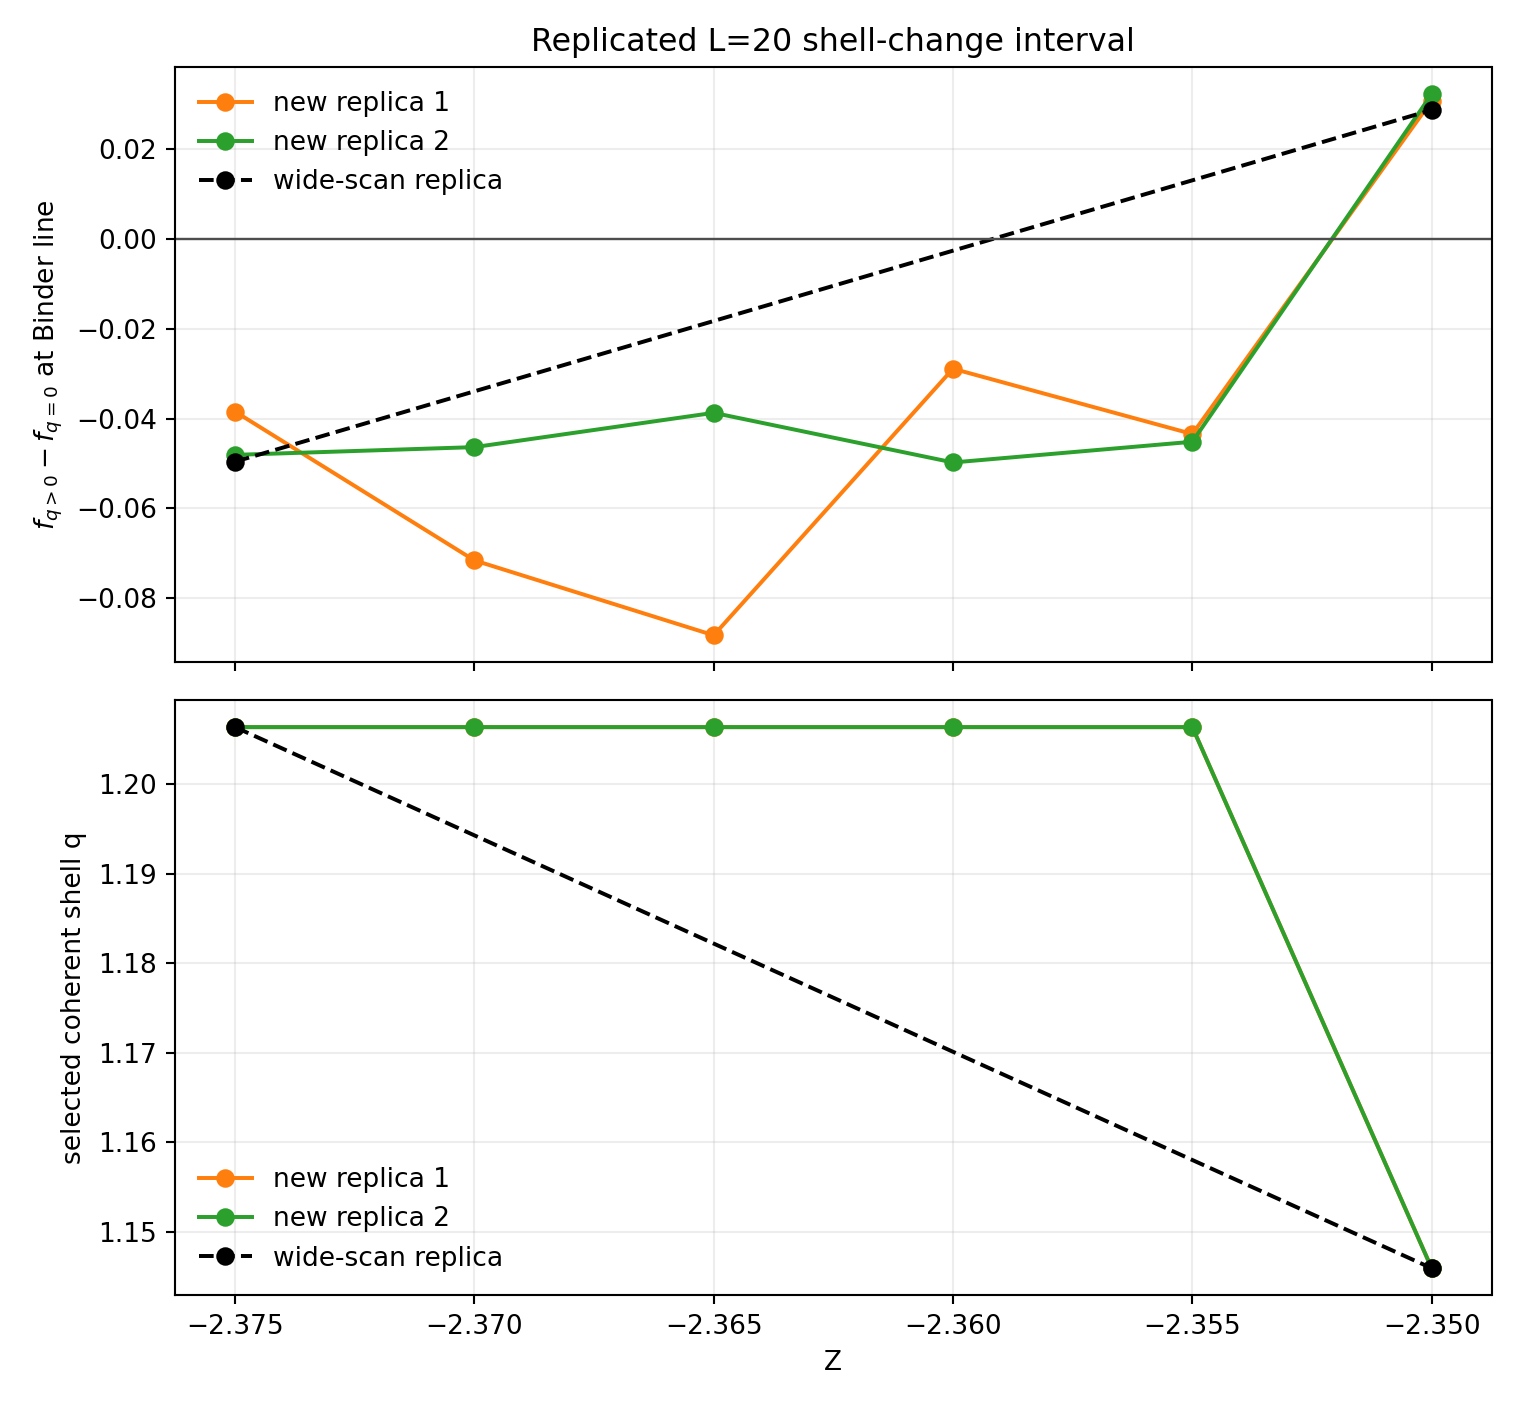
\includegraphics[width=0.82\textwidth]{../structure_factor_cpu/thermodynamic_integration_L20_refine/replicated_onset.png}
  \caption{Replicated refinement of the first $L=20$ sign change.  Both fresh
  replicas switch free-energy sign and selected shell between $Z=-2.350$ and
  $-2.355$.  Their interpolated roots track the deterministic shell midpoint
  in Eq.~\eqref{eq:l20-shell-midpoint}.}
  \label{fig:l20-refine}
\end{figure}

\subsection{Multi-shell envelope and candidate junction with the Binder line}

The single-shell calculations reveal a finite-$q$ region but also demonstrate
that selecting only the lattice shell nearest $-Z/2$ can manufacture sharp
onsets.  To remove this preselection, a new $L=20$ campaign follows five
neighboring nonzero shells independently at every $(Z,m^2)$, together with
uniform and high-mass continuations.  Their free energies share the same
high-mass anchor, and the lowest coherent branch with $S_{\rm peak}\geq10$
defines the finite-$q$ envelope.  The scan covers
$Z=-0.5,-0.625,\ldots,-2.5$ with $\Delta m^2=0.2$ and contains 4382
seven-branch measurements.  Its minimum and mean HMC acceptances are $0.887$
and $0.975$.

Figure~\ref{fig:multishell-connection} shows a much cleaner connection than the
single-shell map.  The finite-$q$ envelope remains above the extrapolated
Binder line through $Z=-1.5$ and below it for every sampled $Z\leq-1.625$:
\begin{equation}
  \Delta f_{\rm Binder}(-1.5)=+0.01165,
  \qquad
  \Delta f_{\rm Binder}(-1.625)=-0.01328.
\end{equation}
The selected shell is $q=0.824429495415$ on both sides, so this sign change is
not a discrete shell switch.  The $q=0$/finite-$q$ equality line crosses the
negative-$Z$ Binder extrapolation at the same location, while at less-negative
$Z$ it lies at higher mass and leaves a candidate modulated wedge before the
finite-$q$ coherence proxy is lost.

\begin{figure}[htbp]
  \centering
  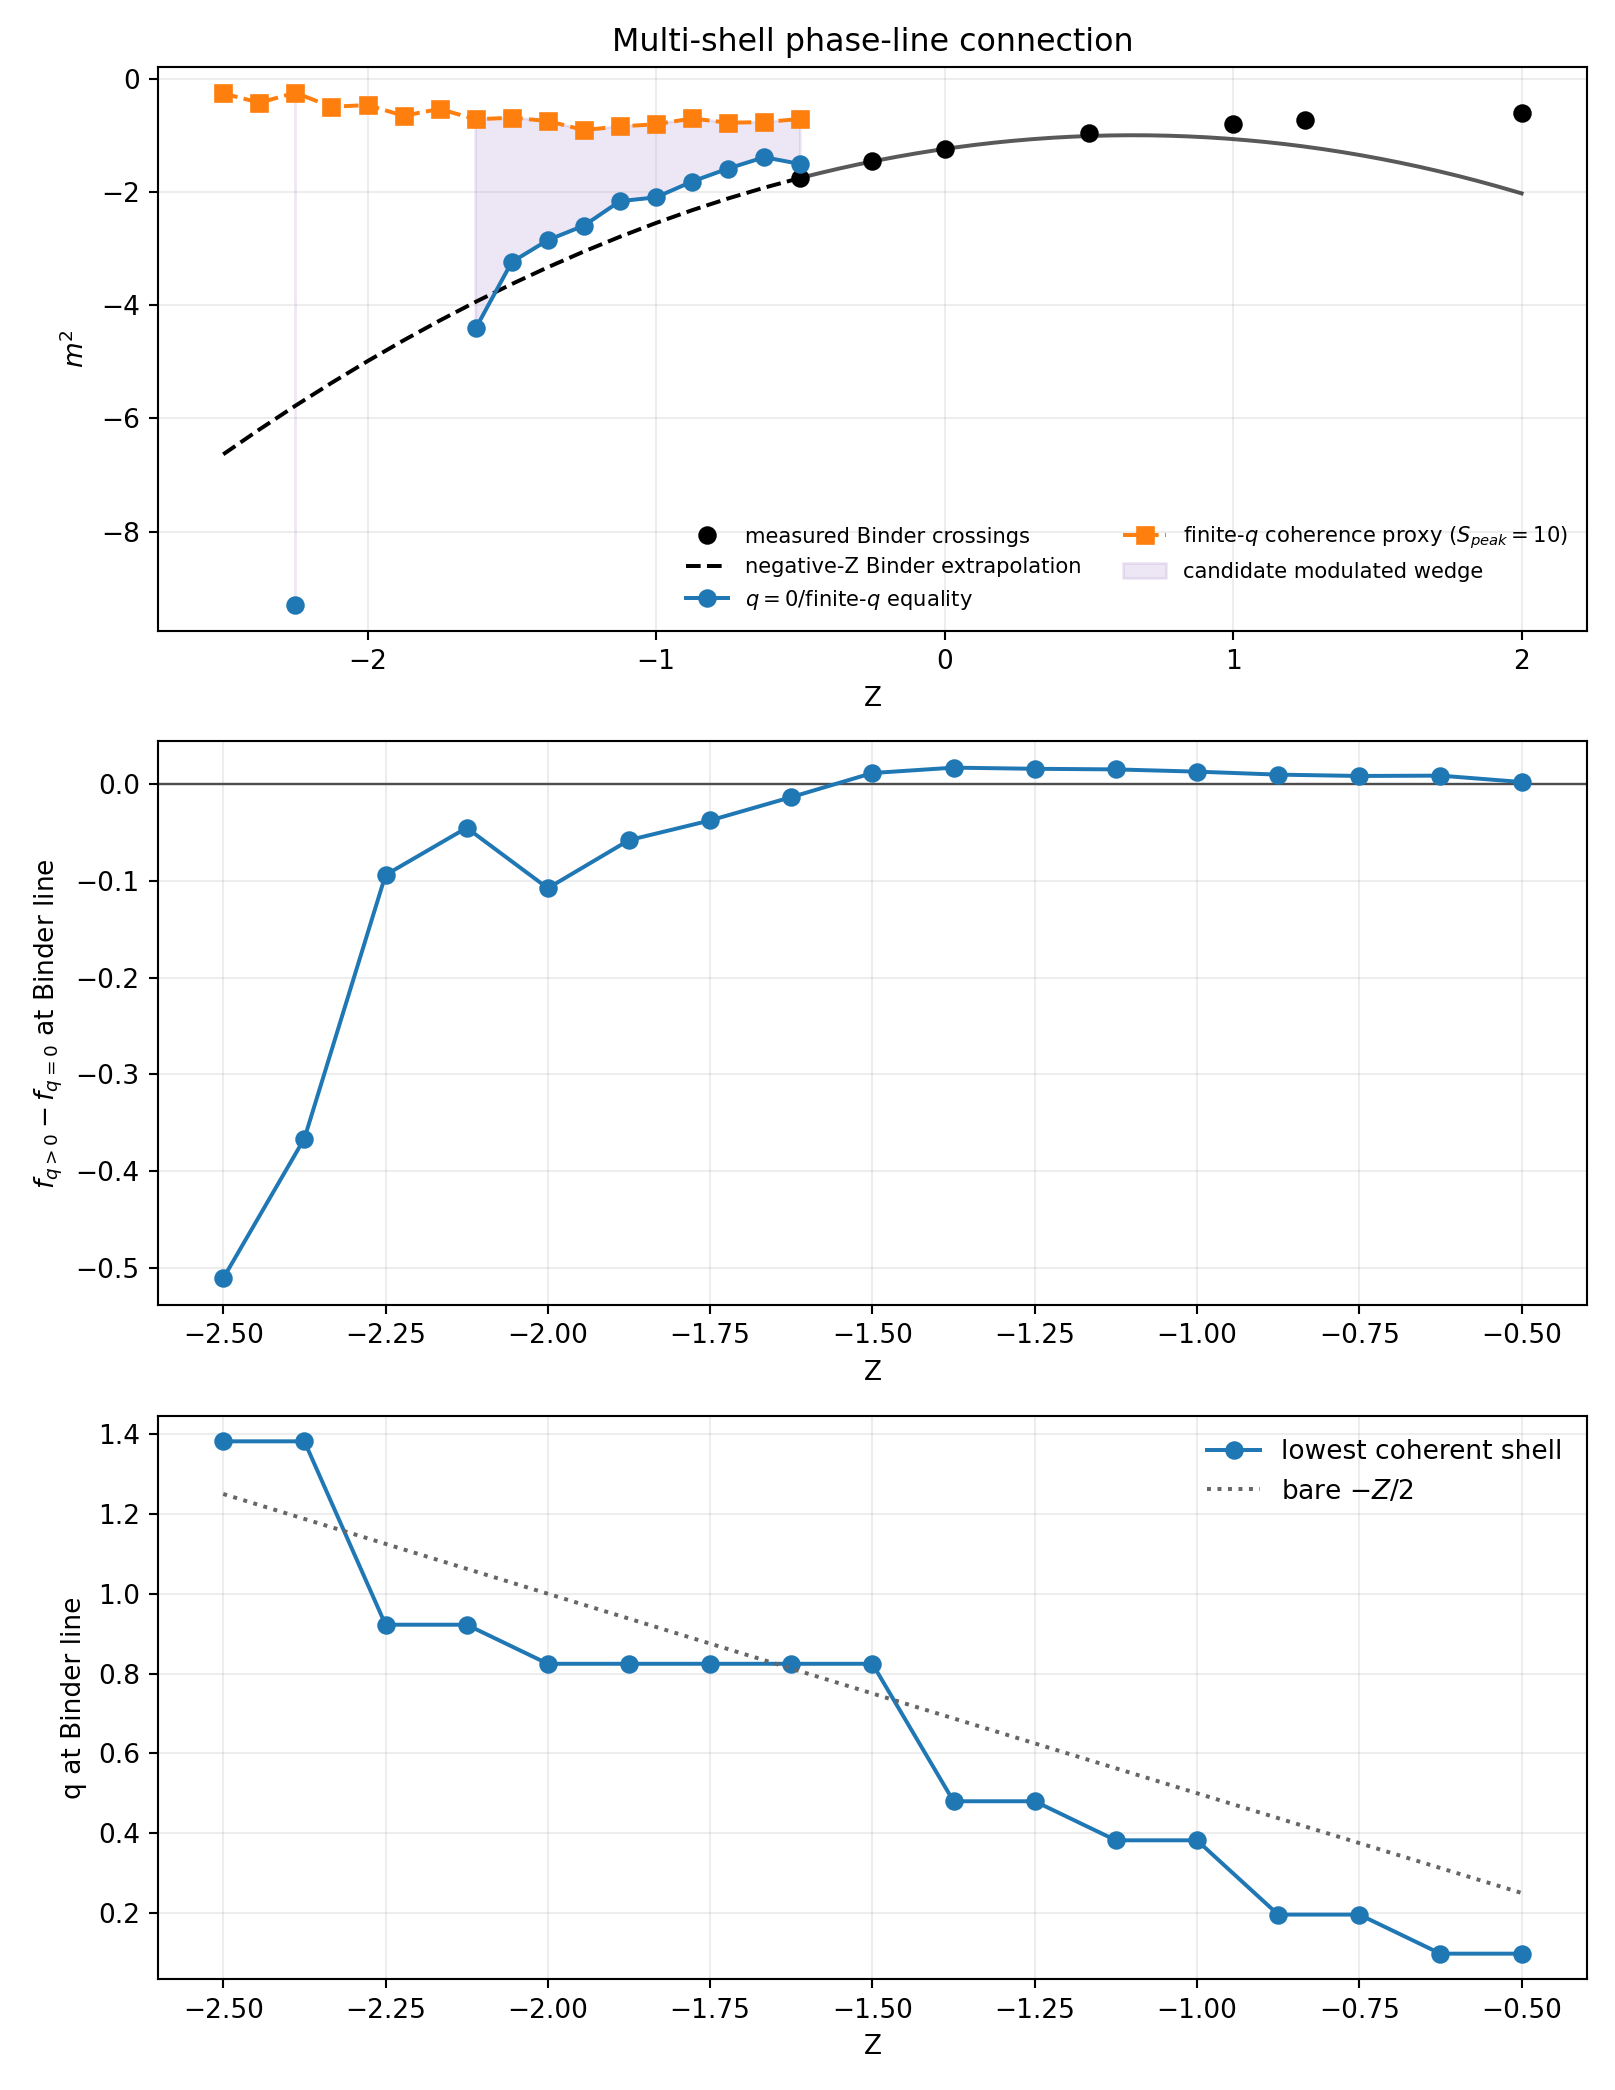
\includegraphics[width=0.84\textwidth]{../structure_factor_cpu/thermodynamic_integration_multishell_L20/phase_line_connection.png}
  \caption{Five-shell phase-line connection at $L=20$.  Top: measured Binder
  crossings, their negative-$Z$ extrapolation, the uniform--finite-$q$
  equality line, and the operational coherence limit.  Middle: envelope free
  energy on the extrapolated Binder line.  Bottom: selected shell.}
  \label{fig:multishell-connection}
\end{figure}

The junction was then rerun with two fresh replicas on
$Z=-1.45,-1.475,\ldots,-1.65$.  Replica~1 changes sign in
$[-1.600,-1.575]$ and gives the linear root $-1.58589$; replica~2 changes sign
in $[-1.550,-1.525]$ and gives $-1.54662$.  The coarse result is approximately
$-1.558$.  As shown in Fig.~\ref{fig:multishell-junction}, the winning shell is
the same $q=0.824429495415$ at every point in both replicas.  The spread between
replicas is nevertheless much larger than the pointwise MCSEs, exposing a
continuation-history systematic.  A conservative statement is therefore
\begin{equation}
  Z_{\rm join}(L=20)\simeq-1.57,
  \qquad -1.60\lesssim Z_{\rm join}\lesssim-1.525
  \quad\text{(continuation systematic)}.
  \label{eq:multishell-junction}
\end{equation}

\begin{figure}[htbp]
  \centering
  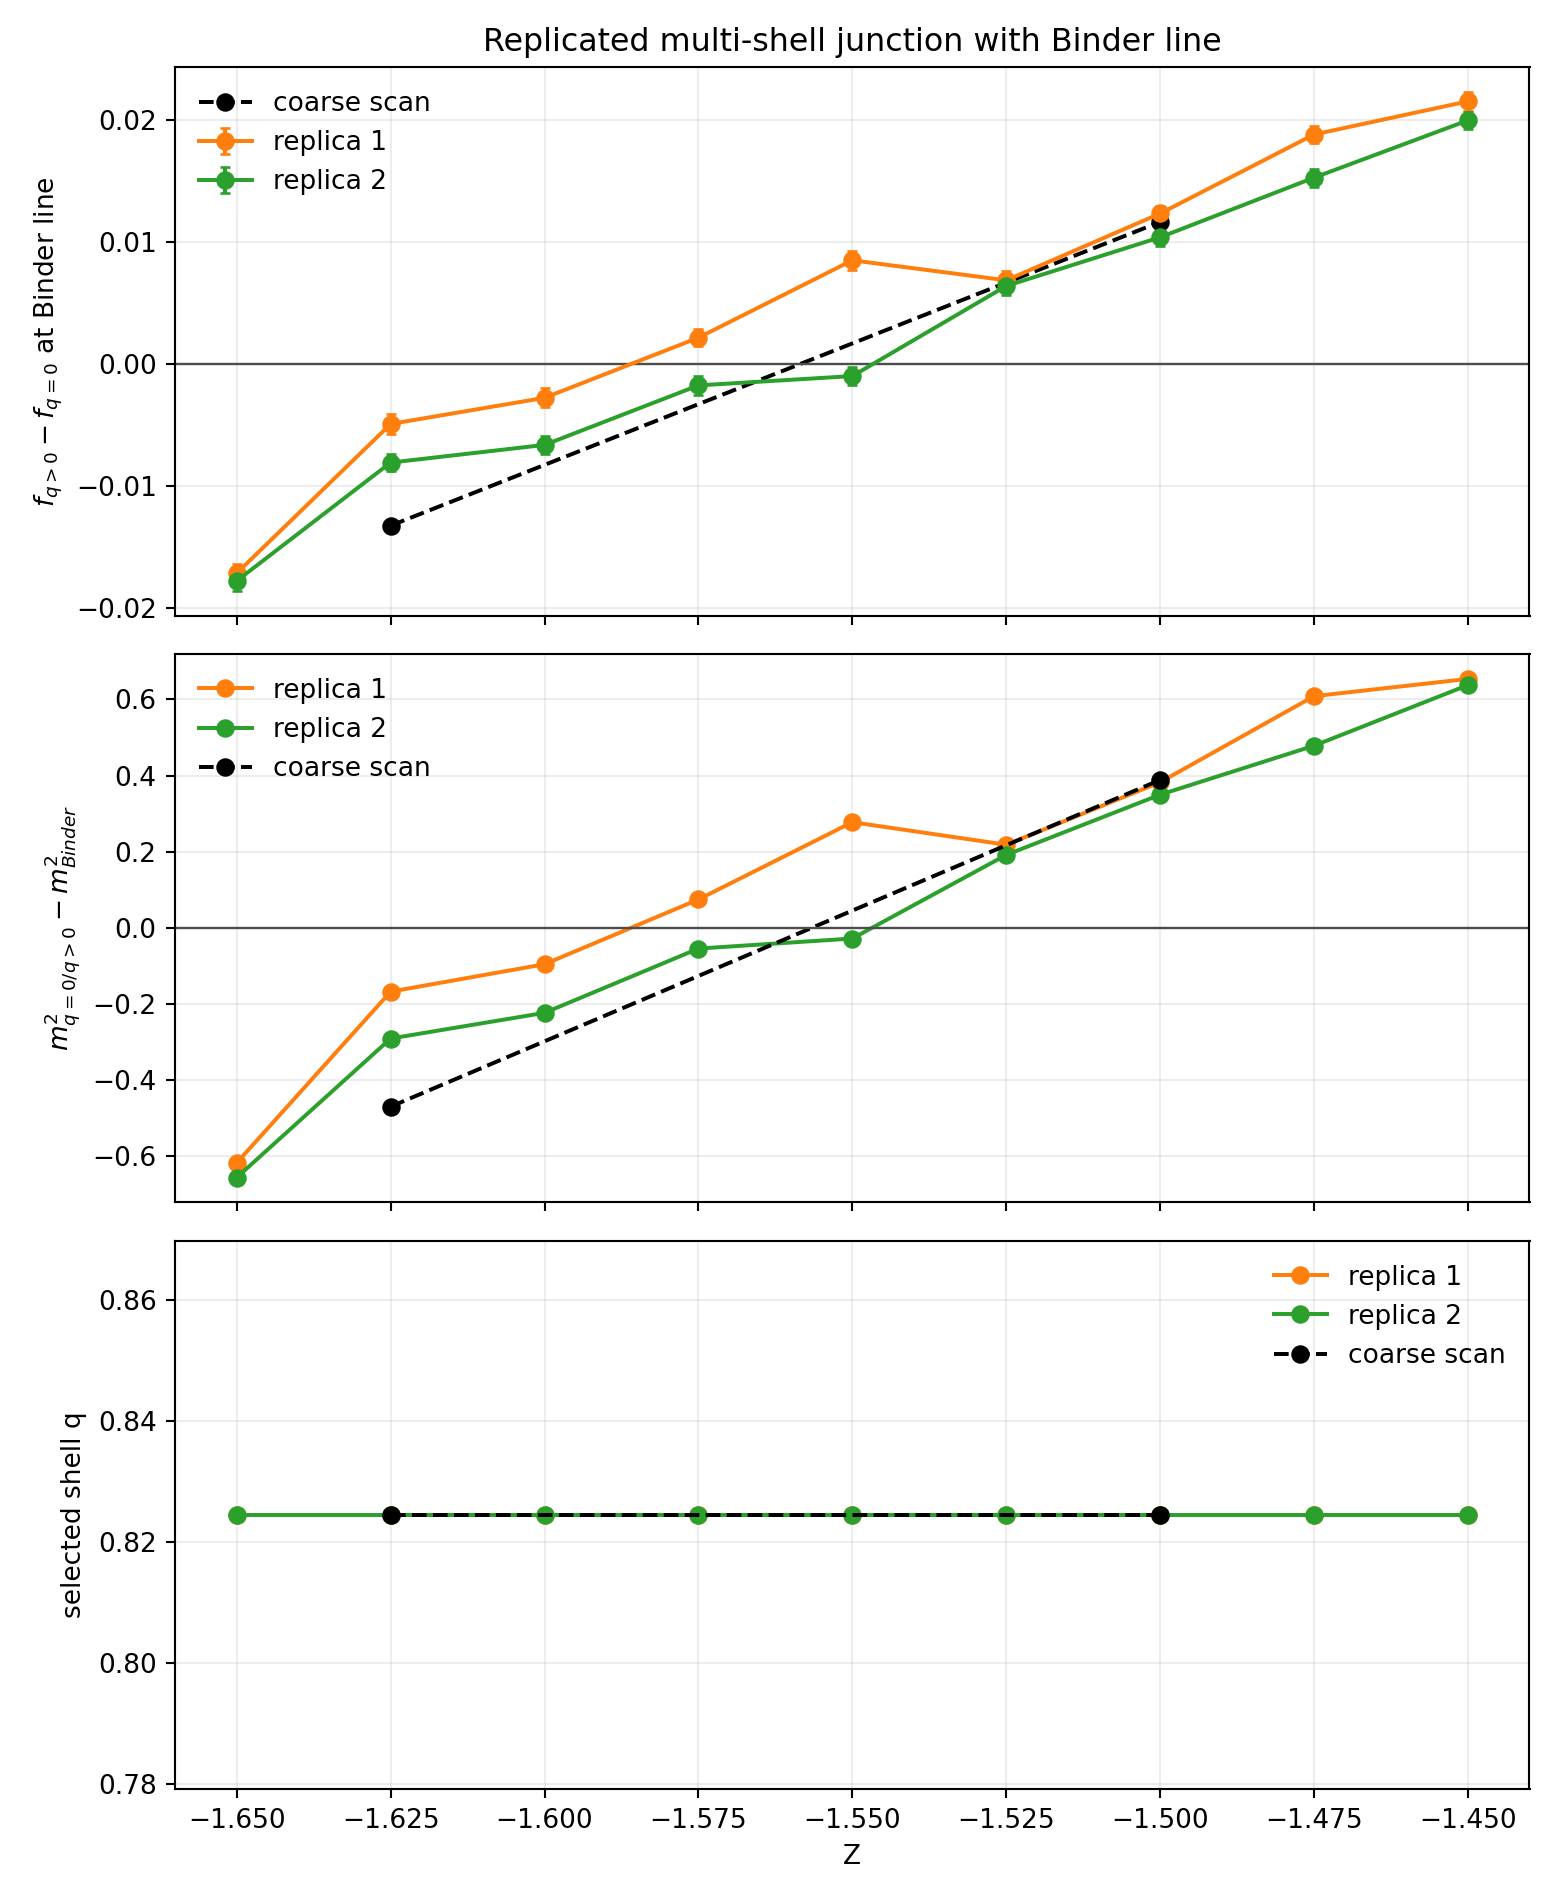
\includegraphics[width=0.82\textwidth]{../structure_factor_cpu/thermodynamic_integration_multishell_join_L20/binder_line_junction.png}
  \caption{Replicated multi-shell junction.  Top: finite-$q$ envelope minus
  uniform free energy on the Binder extrapolation.  Middle: separation between
  the uniform--finite-$q$ equality line and Binder line.  Bottom: the stable
  selected shell, demonstrating that the crossing is not a shell switch.}
  \label{fig:multishell-junction}
\end{figure}

This is the first continuation result consistent with an inhomogeneous branch
joining the uniform transition line without an accompanying shell jump.  It is
not yet a classification of the junction.  The Binder curve is measured only
through $Z=-0.5$ and is quadratically extrapolated over more than one unit in
$Z$; moreover, the branch-history spread in
Eq.~\eqref{eq:multishell-junction} is substantial.  Direct Binder calculations
near the candidate interval, finite-size repetition of the multi-shell
envelope, and a joint reconstruction that allows transitions among shells are
required before distinguishing a Lifshitz point, critical endpoint,
tricritical junction, or metastable continuation artifact.

\section{Reproducibility and data provenance}

The numerical statements in this report are derived from the following local
artifacts:
\begin{itemize}
  \item \path{plots/binder_crossings_vs_Z.csv} and
        \path{plots/binder_crossings_vs_Z.png};
  \item \path{plots/umbrella_binder_mZ*_overlay.png} and the corresponding
        \path{plots/umbrella_binder_mZ*.csv} files;
  \item \path{plots/umbrella_PM2_Zm0p5_m2-1.75.png};
  \item \path{runs/umbrella_binder_Zm0p75/L*/manifest.csv} and
        \path{runs/umbrella_binder_Zm1/L*/manifest.csv};
  \item the analysis implementations
        \path{scripts/umbrella_binder_campaign.py} and
        \path{scripts/plot_binder_crossings_vs_z.py};
  \item the derivative/FSS implementation
        \path{scripts/analyze_binder_slopes.py}, with central validation
        outputs in \path{reports/binder_slope_fss/preliminary/}.
  \item the CPU finite-wavevector implementation
        \path{scripts/structure_factor_campaign.py} and
        \path{scripts/structure_factor_observables.jl}, with staged outputs in
        \path{reports/structure_factor_cpu/}.
  \item the wide continuation implementation
        \path{scripts/thermodynamic_integration_L16.jl} and
        \path{scripts/run_thermodynamic_integration_L16_wide.py}, with the
        manifest, integrated tables, and figures in
        \path{reports/structure_factor_cpu/thermodynamic_integration_L16_wide/}.
  \item the replicated finite-size check
        \path{scripts/run_thermodynamic_integration_L20_onset.py}, with outputs
        in
        \path{reports/structure_factor_cpu/thermodynamic_integration_L20_onset/}.
  \item the wide and refined $L=20$ campaigns
        \path{scripts/run_thermodynamic_integration_L20_wide.py} and
        \path{scripts/run_thermodynamic_integration_L20_refine.py}, with outputs
        in the corresponding
        \path{reports/structure_factor_cpu/thermodynamic_integration_L20_*/}
        directories.
  \item the multi-shell phase-line and replicated junction campaigns
        \path{scripts/run_multishell_phase_map_L20.py} and
        \path{scripts/run_multishell_join_refine_L20.py}, with outputs in
        \path{reports/structure_factor_cpu/thermodynamic_integration_multishell_*/}.
\end{itemize}
The working tree contains ongoing research changes and generated campaign
outputs.  This report records a dated analysis snapshot; it is not a claim
that the repository state is a frozen release.

\section{Conclusion}

The calculations now separate three related signals.  First, the transition
location in $m^2$ inferred from uniform Binder crossings is comparatively
stable across adjacent sizes, while the crossing value is not.  Second, the
completed structure-factor campaign directly finds nonzero-shell dominance at
$Z=-1$ for $L=16,20$, and the deep $Z=-4$ calibration confirms that the
estimator is robust against phase and orientational averaging.  Third, the
wide $L=16$ continuation map shows a restricted free-energy change on the
extrapolated Binder line between $Z=-2.275$ and $-2.300$; however, two
independent $L=20$ replicas remain uniformly on the $q=0$ side throughout the
same interval.  The extended $L=20$ scan develops its own sign change near
$Z=-2.3521$, but this value follows the midpoint between two discrete momentum
shells with striking precision.  Allowing five nearby shells to compete
removes that artifact and instead identifies a candidate connection to the
Binder extrapolation near $Z\simeq-1.57$, with a continuation-systematic range
approximately $[-1.60,-1.525]$ and no shell change across the junction.

The $L=16$ bracket is therefore not a thermodynamic critical point.  It
coincides with a discrete change of the favored momentum shell and fails the
first finite-size replication; the analogous $L=20$ crossing is itself pinned
to a shell switch.  The present results remain direct evidence for a
finite-wavevector regime and for the inadequacy of a purely uniform order
parameter, but they do not establish a first-order boundary, critical endpoint,
Lifshitz point, or tricritical point.  The immediate priority is direct Binder
sampling near $Z\simeq-1.57$, because the present uniform line is only
extrapolated there, followed by repeating the multi-shell construction at a
third volume and enabling actual transitions among competing shells before
coexistence and barrier scaling.

\begin{thebibliography}{9}

\bibitem{Hornreich1975}
R.~M. Hornreich, M. Luban, and S. Shtrikman,
``Critical behavior at the onset of $k$-space instability on the $\lambda$
line,'' \emph{Phys. Rev. Lett.} \textbf{35}, 1678--1681 (1975).
\href{https://doi.org/10.1103/PhysRevLett.35.1678}
{doi:10.1103/PhysRevLett.35.1678}.

\bibitem{Binder1981}
K. Binder,
``Finite size scaling analysis of Ising model block distribution functions,''
\emph{Z. Phys. B} \textbf{43}, 119--140 (1981).
\href{https://doi.org/10.1007/BF01293604}{doi:10.1007/BF01293604}.

\bibitem{Duane1987}
S. Duane, A.~D. Kennedy, B.~J. Pendleton, and D. Roweth,
``Hybrid Monte Carlo,'' \emph{Phys. Lett. B} \textbf{195}, 216--222 (1987).
\href{https://doi.org/10.1016/0370-2693(87)91197-X}
{doi:10.1016/0370-2693(87)91197-X}.

\bibitem{Ferrenberg2018}
A.~M. Ferrenberg, J. Xu, and D.~P. Landau,
``Pushing the limits of Monte Carlo simulations for the three-dimensional
Ising model,'' \emph{Phys. Rev. E} \textbf{97}, 043301 (2018).
\href{https://doi.org/10.1103/PhysRevE.97.043301}
{doi:10.1103/PhysRevE.97.043301}.

\bibitem{Hasenbusch1999}
M. Hasenbusch, K. Pinn, and S. Vinti,
``Critical exponents of the three-dimensional Ising universality class from
finite-size scaling with standard and improved actions,''
\emph{Phys. Rev. B} \textbf{59}, 11471--11483 (1999).
\href{https://doi.org/10.1103/PhysRevB.59.11471}
{doi:10.1103/PhysRevB.59.11471}.

\bibitem{Stephen1975}
M.~J. Stephen, E. Abrahams, and J.~P. Straley,
``Logarithmic corrections to the mean-field theory of tricritical points,''
\emph{Phys. Rev. B} \textbf{12}, 256--262 (1975).
\href{https://doi.org/10.1103/PhysRevB.12.256}
{doi:10.1103/PhysRevB.12.256}.

\end{thebibliography}

\end{document}
